%%%%%%%%%%%%%%
%% Run LaTeX on this file several times to get Table of Contents,
%% cross-references, and citations.

%% If you have font problems, you may edit the w-bookps.sty file
%% to customize the font names to match those on your system.

%% w-bksamp.tex. Current Version: Feb 16, 2012
%%%%%%%%%%%%%%%%%%%%%%%%%%%%%%%%%%%%%%%%%%%%%%%%%%%%%%%%%%%%%%%%
%
%  Sample file for
%  Wiley Book Style, Design No.: SD 001B, 7x10
%  Wiley Book Style, Design No.: SD 004B, 6x9
%
%
%  Prepared by Amy Hendrickson, TeXnology Inc.
%  http://www.texnology.com
%%%%%%%%%%%%%%%%%%%%%%%%%%%%%%%%%%%%%%%%%%%%%%%%%%%%%%%%%%%%%%%%

%%%%%%%%%%%%%
% 7x10
%\documentclass{wileySev}

% 6x9
\documentclass{wileySix}

\usepackage{graphicx}
\usepackage{listings}

\usepackage{color}
 
\definecolor{codegreen}{rgb}{0,0.6,0}
\definecolor{codegray}{rgb}{0.5,0.5,0.5}
\definecolor{codepurple}{rgb}{0.58,0,0.82}
\definecolor{backcolour}{rgb}{0.95,0.95,0.92}
 
\lstdefinestyle{mystyle}{
    backgroundcolor=\color{backcolour},   
    commentstyle=\color{codegreen},
    keywordstyle=\color{magenta},
    numberstyle=\tiny\color{codegray},
    stringstyle=\color{codepurple},
    basicstyle=\footnotesize,
    breakatwhitespace=false,         
    breaklines=true,                 
    captionpos=b,                    
    keepspaces=true,                 
    numbers=left,                    
    numbersep=5pt,                  
    showspaces=false,                
    showstringspaces=false,
    showtabs=false,                  
    tabsize=2,
    language=sh
}
 
\lstset{style=mystyle}

%%%%%%%
%% for times math: However, this package disables bold math (!)
%% \mathbf{x} will still work, but you will not have bold math
%% in section heads or chapter titles. If you don't use math
%% in those environments, mathptmx might be a good choice.

% \usepackage{mathptmx}

% For PostScript text
\usepackage{w-bookps}

%%%%%%%%%%%%%%%%%%%%%%%%%%%%%%%%%%%%%%%%%%%%%%%%%%%%%%%%%%%%%%%%
%% Other packages you might want to use:

% for chapter bibliography made with BibTeX
% \usepackage{chapterbib}

% for multiple indices
% \usepackage{multind}

% for answers to problems
% \usepackage{answers}

%%%%%%%%%%%%%%%%%%%%%%%%%%%%%%
%% Change options here if you want:
%%
%% How many levels of section head would you like numbered?
%% 0= no section numbers, 1= section, 2= subsection, 3= subsubsection
%%==>>
\setcounter{secnumdepth}{3}

%% How many levels of section head would you like to appear in the
%% Table of Contents?
%% 0= chapter titles, 1= section titles, 2= subsection titles, 
%% 3= subsubsection titles.
%%==>>
\setcounter{tocdepth}{2}

%% Cropmarks? good for final page makeup
%% \docropmarks

%%%%%%%%%%%%%%%%%%%%%%%%%%%%%%
%
% DRAFT
%
% Uncomment to get double spacing between lines, current date and time
% printed at bottom of page.
% \draft
% (If you want to keep tables from becoming double spaced also uncomment
% this):
% \renewcommand{\arraystretch}{0.6}
%%%%%%%%%%%%%%%%%%%%%%%%%%%%%%

%%%%%%% Demo of section head containing sample macro:
%% To get a macro to expand correctly in a section head, with upper and
%% lower case math, put the definition and set the box 
%% before \begin{document}, so that when it appears in the 
%% table of contents it will also work:

\newcommand{\VT}[1]{\ensuremath{{V_{T#1}}}}

%% use a box to expand the macro before we put it into the section head:

\newbox\sectsavebox
\setbox\sectsavebox=\hbox{\boldmath\VT{xyz}}

%%%%%%%%%%%%%%%%% End Demo


\begin{document}


\booktitle{Cerdas Menguasai Python}
\subtitle{Dalam 24 Jam}

\authors{Rolly M. Awangga\\
\affil{Informatics Research Center}
%Floyd J. Fowler, Jr.\\
%\affil{University of New Mexico}
}

\offprintinfo{Cerdas Menguasai Python, First Edition}{Rolly M. Awangga}

%% Can use \\ if title, and edition are too wide, ie,
%% \offprintinfo{Survey Methodology,\\ Second Edition}{Robert M. Groves}

%%%%%%%%%%%%%%%%%%%%%%%%%%%%%%
%% 
\halftitlepage

\titlepage


\begin{copyrightpage}{2019}
%Survey Methodology / Robert M. Groves . . . [et al.].
%\       p. cm.---(Wiley series in survey methodology)
%\    ``Wiley-Interscience."
%\    Includes bibliographical references and index.
%\    ISBN 0-471-48348-6 (pbk.)
%\    1. Surveys---Methodology.  2. Social 
%\  sciences---Research---Statistical methods.  I. Groves, Robert M.  II. %
%Series.\\
%
%HA31.2.S873 2007
%001.4'33---dc22                                             2004044064
\end{copyrightpage}

\dedication{`Jika Kamu tidak dapat menahan lelahnya belajar, 
Maka kamu harus sanggup menahan perihnya Kebodohan.'
~Imam Syafi'i~}

\begin{contributors}
\name{Rolly Maulana Awangga,} Informatics Research Center., Politeknik Pos Indonesia, Bandung,
Indonesia



\end{contributors}

\contentsinbrief
\tableofcontents
\listoffigures
\listoftables
\lstlistoflistings


\begin{foreword}
Sepatah kata dari Kaprodi, Kabag Kemahasiswaan dan Mahasiswa
\end{foreword}

\begin{preface}
Buku ini diciptakan bagi yang awam dengan git sekalipun.

\prefaceauthor{R. M. Awangga}
\where{Bandung, Jawa Barat\\
Februari, 2019}
\end{preface}


\begin{acknowledgments}
Terima kasih atas semua masukan dari para mahasiswa agar bisa membuat buku ini 
lebih baik dan lebih mudah dimengerti.

Terima kasih ini juga ditujukan khusus untuk team IRC yang 
telah fokus untuk belajar dan memahami bagaimana buku ini mendampingi proses 
Intership.
\authorinitials{R. M. A.}
\end{acknowledgments}

\begin{acronyms}
\acro{ACGIH}{American Conference of Governmental Industrial Hygienists}
\acro{AEC}{Atomic Energy Commission}
\acro{OSHA}{Occupational Health and Safety Commission}
\acro{SAMA}{Scientific Apparatus Makers Association}
\end{acronyms}

\begin{glossary}
\term{git}Merupakan manajemen sumber kode yang dibuat oleh linus torvald.

\term{bash}Merupakan bahasa sistem operasi berbasiskan *NIX.

\term{linux}Sistem operasi berbasis sumber kode terbuka yang dibuat oleh Linus Torvald
\end{glossary}

\begin{symbols}
\term{A}Amplitude

\term{\hbox{\&}}Propositional logic symbol 

\term{a}Filter Coefficient

\bigskip

\term{\mathcal{B}}Number of Beats
\end{symbols}

\begin{introduction}

%% optional, but if you want to list author:

\introauthor{Rolly Maulana Awangga, S.T., M.T.}
{Informatics Research Center\\
Bandung, Jawa Barat, Indonesia}

Pada era disruptif  \index{disruptif}\index{disruptif!modern} 
saat ini. git merupakan sebuah kebutuhan dalam sebuah organisasi pengembangan perangkat lunak.
Buku ini diharapkan bisa menjadi penghantar para programmer, analis, IT Operation dan Project Manajer.
Dalam melakukan implementasi git pada diri dan organisasinya.

Rumusnya cuman sebagai contoh aja biar keren\cite{awangga2018sampeu}.

\begin{equation}
ABC {\cal DEF} \alpha\beta\Gamma\Delta\sum^{abc}_{def}
\end{equation}

\end{introduction}

%%%%%%%%%%%%%%%%%%Isi Buku_

\chapter{SEJARAH DAN KARAKTERISTIK  PYTHON}

\section{Resume}
\subsection{Resume Sejarah Python}
\begin{flushleft}
\qquad Bahasa pemrograman Python dirilis pertama kali oleh Guido van Rossum di tahun 1991, yang sudah dikembangkan sejak tahun 1989. Awal pemilihan nama Python tidak secara langsung berasal dari nama ular piton, tapi sebuah acara humor di BBC pada era 1980an dengan judul “Monty Python’s Flying Circus“. Monty Python adalah kelompok lawak yang membawakan acara tersebut. Kebetulan Guido van Rossum adalah penggemar dari acara ini. Pada tahun 1994, Python 1.0 dirilis, yang diikuti dengan Python 2.0 pada tahun 2000. Python 3.0 keluar pada tahun 2008.
\end{flushleft}
\subsection{Perbedaan Python 2 dan Python 3}
\subsubsection{Python 2}
\paragraph{}
Dipublikasikan pada akhir tahun 2000, Python 2 dinilai lebih transparan dan inklusif untuk pengembangan software ketimbang versi sebelumnya. Hal ini didukung dengan adanya PEP – Python Enhancement Proposal, sebuah spesifikasi teknis yang menjadi tuntunan informasi untuk penggunanya dan menggambarkan fitur baru pada Python itu sendiri. Sebagai tambahan, Python 2 dilengkapi dengan berbagai fitur programatikal seperti cycle-detecting garbage collector untuk mengotomasi manajemen memori, peningkatan dukungan untuk Unicode, list comprehension untuk membuat sebuah list berdasarkan list yang sudah ada. Unifikasi pada tipe data Python dan class ke satu hirarki terjadi pada rilis Python 2.2
\subsubsection{Python 3}
\paragraph{}
Python 3 diharapkan sebagai masa depan Python dan merupakan versi yang saat tulisan ini dibuat masih aktif dikembangkan. Python 3 sendiri adalah versi dengan banyak perubahan yang dirilis akhir tahun 2008. Fokus dari Python 3 itu sendiri adalah untuk melakukan perapian pada codebase dan menghapuskan duplikasi (redundancy). Perubahan terbesar pada Python 3 termasuk memasukkan statemen print ke dalam built-in function. Awalnya, Python 3 mengalami hambatan pada pengadopsiannya. Itu akibat dari tidak adanya backwards compatibility dengan Python 2. Hal ini membuat pengguna Python sangat berat hati untuk pindah ke versi 3 ini. Tambahannya, banyak sekali library yang hanya tersedia untuk Python 2., tapi setelah tim pengembangan di balik Python 3 telah berulang kali menjelaskan bahwa dukungan terhadap Python 2 akan segera dihentikan, dan semakin banyak libary disalin ke Python 3, maka penerapan Python 3 semakin lama semakin meningkat.
\subsection{Implementasi dan penggunaan Python pada Perusahaan}
daftar berikut adalah beberapa perusahaan yang menggunakan Python, diantaranya:
\begin{enumerate}
\item
Google adalah perusahaan besar yang menggunakan banyak kode Python di dalam mesin pencarinya. Dan mesin pencari google adalah yang paling terkenal di dunia.
\item
Youtube, situs video terbesar dan terpopuler di dunia, sebagian besar kodenya ditulis dalam bahasa Python.
\item
Facebook, media sosial terbesar di dunia, menggunakan Tornado, sebuah framework Python untuk menampilkan timeline.
\item
Instagram, siapa yang tidak kenal. Instagram menggunakan Django, framework python sebagai mesin pengolah sisi server dari aplikasinya.
\item
Pinterest, banyak menggunakan python untuk membangun aplikasinya.
\item
Dropbox, barangkali Anda adalah salah seorang pengguna layanan ini. Dropbox menggunakan python baik di sisi server maupun di sisi pengguna layanannya.
\item
Quora, salah satu situs tanya jawab terbesar di dunia, dibangun menggunakan Python.
\item
NASA, badan antariksa Amerika ini menggunakan Python untuk bidang sainsnya.
\item
NSA, badan mata – mata Amerika banyak menggunakan Python untuk analisa kriptografi dan intelijen.
\item
Blender, Maya, software pembuat animasi 3D terkenal, menggunakan Python sebagai salah satu bahasa skrip pemrogramannya.
\item
Raspberry Pi, komputer mini yang banyak digunakan sebagai mikrokontroller, menggunakan Python sebagai bahasa utamanya.
\end{enumerate}


\section{Instalasi}
\subsection{Cara Pemakaian Script dan interpreter python}
\subsection{Cara Pemakaian spyder termasuk variable explorer}

\section{Mencoba Python}
Untuk memulai suatu pemrograman, kita akan awali dengan membuat sebuah hello world. Di Python, cukup mudah untuk membuat sebuah hello world. Silahkan buat sebuah file dengan nama helloworld.py kemudian buat kode berikut di dalam file tersebut:
\paragraph{}
print "Hello world..."
\paragraph{}
Sekarang mari kita eksekusi file tersebut di konsol dengan perintah berikut:
python helloworld.py
\paragraph{}
Hello world...

\section{Identasi}
Ketika menulis kode program Python perlu memperhatikan indentasi, karena kode program Python distrukturkan berdasarkan indentasi. Kode program yang berada pada sisi kiri yang sama maka dibaca sebagai satu blok, untuk membuat sub blok maka cukup dengan memberikan jarak spasi atau tab ke kanan.
Soal indentasi ini akan lebih jelas ketika pembahasan tentang pencabangan, perulangan, fungsi, class, dan materi yang lain yang membutuhkan penulisan kode program bersarang.
Contohnya adalah sebagai berikut:
import sys
\paragraph{}
if len(sys.argv) < 2:
\paragraph{}
    print("Harap memasukkan argumen.")
    \paragraph{}
    sys.exit(1)
	
	\section{AlvanAlvanzah/1174077}
\subsection{Background}
Python adalah bahasa pemrograman interpretatif multiguna dengan filosofi perancangan yang berfokus pada tingkat keterbacaan kode. Python diklaim dijadikan bahasa yang menggabungkan kapabilitas, kesanggupan, dengan sintaksis kode yang sangat jelas, dan dilengkapi dengan fungsionalitas pustaka standar yang besar serta komprehensif.
\par
Python adalah bahasa pemrograman yang bersifat open source. Bahasa pemrograman ini dioptimalisasikan untuk software quality, developer productivity, program portability, dan component integration. Python telah digunakan untuk mengembangkan berbagai macam perangkat lunak, seperti internet scripting, systems programming, user interfaces, product customization, numberic programming dll. Python saat ini telah menduduki posisi 4 atau 5 bahasa pemrograman paling sering digunakan di seluruh dunia. Menggunakan alat pihak ketiga, kode Python dapat dikemas ke dalam program yang dapat dieksekusi mandiri. Penerjemah python tersedia untuk banyak sistem operasi.
\subsection{Problems}
\begin{itemize}
\item Bagaimana cara agar memahami bahasa pemrograman python
\end{itemize}
\subsection{Objective and Contribution}
\subsubsection{Objective}
\begin{itemize}
\item Dapat memahami bahasa pemrograman Python
\end{itemize}
\subsubsection{Contribution}
\begin{itemize}
\item Dapat mengimplementasikan bahasa pemrograman python
\end{itemize}

\subsection{Scoop and Environtment}
\begin{itemize}
\item Mempelajari tentang bahasa pemrograman python
\end{itemize}


\chapter{Pemrograman Dasar}
\section{Perintah Navigasi}
Perintah navigasi direktori


\chapter{Fungsi dan Kelas}
\section {Sekar }

\documentclass[10pt]{article}

\title{Fungsi}

\begin{document}
Pada contoh dibawah , sebuah fungsi dengan nama perkalian(), memiliki dua buah argumen yaitu a dan b. Isi dari fungsi tersebut adalah melakukan perhitungan perkalian yang diambil dari nilai a dan b, yang di simpan ke dalam variabel c. Nilai dari c lah yang akan dikembalikan oleh fungsi dari hasil pemanggilan fungsi melalui statemen perkalian(5,10)\\
\include 
\begin{equation}
Contoh:\\
def perkalian(a,b):
	c = a*b
return c
	#Program Utama
print( perkalian(5,10))

>>> def nama():
	gelar = 'Mr'
	aksi = (lambda x: gelar + ' ' + x)
	return aksi

>>> act = nama()
>>> act('Namjoon')
'Sir Namjoon'
\end{equation}

\begin{Scope Variabel}
cakupan variabel merupakan suatu keadaan dimana pendeklarasian sebuah variabel di tentukan , Dalam scope variabel dikenal dua istilah yaitu local dan global.
Contoh penggunaan scope variabel() :
x = 12
y = 3
	print "Sebelum memanggil fungsi, x bernilai", x
	print "Sebelum memanggil fungsi, y bernilai", y
swap(x,y)
	print "Setelah memanggil fungsi, x bernilai", x
	print "Setelah memanggil fungsi, y bernilai", y
	
\begin{Fungsi Rekursif}
untuk menyederhanakan penulisan program dan menggantikan bentuk iterasi. Dengan rekursi, program akan lebih mudah dilihat.
# Fungsi Rekursif faktorial
	def faktorial(nilai):
		if nilai <= 1:
	return 1
		else:
	return nilai * faktorial(nilai - 1)
#Program utama
	for i in range(11):
	print "%2d ! = %d" % (i, faktorial(i))
	
\begin{Melewatkan Argumen dengan Kata Kunci}
Jika fungsi perkalian kita panggil dengan memberi pernyataan perkalian(10,8), maka nilai 10 akan disalin ke variabel x dan nilai 8 ke variabel y.\\
def perkalian(a, b):
	"Mengalikan dua bilangan"
	z = x * y
		print "Nilai a =",a
		print "Nilai b =",b
		print "a* b =",c
# program utama mulai di sini
	perkalian(5,3)
		print perkalian(b=4,a=2)
Hasilnya:
Nilai a = 5
Nilai b = 3
a*b = 15
Nilai a = 2

Jadi nilai default hanya boleh diberikan kepada deretan akhir parameter. Setelah pemberian nilai default, semua parameter di belakangnya juga harus diberi nilai default. Satu catatan, nilai awal argumen akan dievaluasi pada saat dideklarasikan. Perhatikan contoh berikut :
usernm="admin"
passwd="aa"
def login(username=usernm, password=passwd):
	print "Your username ",username
	print "Your password ",password
	print 
	usernm="tamu" 
	passwd="cc"
login()
Untuk memanggil fungsi dengan deklarasi seperti ini, kita harus menyebutkan daftar argumen beserta kata-kuncinya. 
Contoh ():
	def cetak1():
print ‘Hello World’
	def cetak2(n):
print n
	cetak1()
hallo world
	cetak2(123)
123
	cetak2('apa kabar?')
apa kabar
	def cetak3(x,y,z):
print x,y,z
	def cetak4(x,y,z=4):
print x,y,z
	cetak3(1,2,3)
1 2 3
	cetak4(1,2)
1 2 4
	cetak4(1,2,3)
1 2 3

\class Ngitung:
  def __init

\end{document}

\begin{Kelas}
Class adalah salah satu cara bagaimana kita membuat sebuah kode yang mempunyai behaviour tertentu dan lebih mudah dalam mengorganisasi berbagai fungsi dan state-nya. Dalam sebuah class kamu dapat menyimpan sebuah state tanpa harus membuat banyak state bila tidak menggunakan class.\\
Contoh :\\
class Product:
    __vendor_message = "Ini adalah rahasia"
    name = ""
    price = ""
    size = ""
    unit = ""
    
    def __init__(self, name):
        print "Ini adalah constructor"
        self.name = name
        self.unit = "ml"
        self.size = 350
        
    def get_vendor_message(self):
        print self.__vendor_message
        
	def set_price(self, price):
        self.price = price
        
p = Product("Banana Milk")
p.set_price(5500)

print "%s dengan ukuran %s %s harganya Rp. %d" % (p.name, p.size, p.unit, p.price)
# print p.__vendor_message

p.get_vendor_message()

p1 = Product("UltraMilk")
p1.set_price(3000)

print "%s dengan ukuran %s %s harganya Rp. %d" % (p.name, p.size, p.unit, p.price)

print p == p
print p1 == p1
print p == p1

\begin{Pemahanan Teori}
1.void(fungsi tanpa nilai balik)
	Fungsi yang void sering disebut juga prosedur. Disebut void karena fungsi tersebut tidak mengembalikan suatu nilai keluaran yang didapat dari hasil proses tersebut.
	Ciri-ciri dari jenis fungsi Void , yaitu :
	1. tidak adanya keyword return
	2. tidak adanya tipe data di dalam deklarasi fungsi
	3. menggunakan keyword void
	4. tidak memiliki nilai kembalian fungsi
	5. Keyword void juga digunakan jika suatu function tidak 				   mengandung suatu parameter apapun.
Contohnya:\\
	void menampilkan_jumlah(int a, int b)}
		in jumlah;
		jumlah = a + b;
		cout << jumlah;
	}
2.Non void (fungsi dengan nilai balik
	Fungsi non-void disebut juga function . disebut non-void karena mengembalikan nilai kembalian yang berasal dari keluaran hasil proses function tersebut.
	Ciri-ciri dari jenis fungsi Non-Void , yaitu :
	1. Ada keyword return
	2. ada tipe data yang mengawali fungsi
	3. tidak ada keyword void
	4. memiliki nilai keyword
	5. Non-void : int jumlah (int a, int b)

3. Prototype Function
	Sebuah program C++ dapat terdiri dari banyak fungsi. Salah satu fungsi tersebut harus bernama main(). Jika fungsi yang lain dituliskan setelah fungsi main(), sebelum fungsi main ditambahkan.
	Contohnya:\\
#include <stdio.h>
\\prototype function
	int hitung(int angka, int bilangan);
	int tulis(char);
	int tampil(int angka[],char huruf);
//fungsi main
	int main(){
		int array[3]={1,2,3};
		char huruf="D";
		//memanggil fungsi
		hitung (2,3);
		tulis("A");
		tampil(array,huruf);
}

4. Fungsi Rekursif
	Fungsi yang memanggil dirinya sendiri. Artinya , fungsi tersebut dipanggil di dalam tubuh fungsi itu sendiri. Parameter yang dilewatkan berubah sebanyak fungsi itu dipanggil.
	
\begin{Apa itu paket dan cara pemanggilan paket atau library dengan contoh kode program lainnya}
	<?php if ( ! defined('BASEPATH'))
		exit('No direct script access allowed');
	class Blog extends ci_controller {
	function __construct()
	{
		parent ::__construct();
	}
	function index()
	{
		echo "Hallo.. saya min yoongi adalah contoh dari boyband BTS 				yang mendunia";
	}
	
	
}

\begin{Jelaskan Apa itu kelas, apa itu objek, apa itu atribut, apa itu method dan contoh kode program lainnya masing-masing.}
gambaran umum tentang sebuah benda. Di dalam pemrograman nantinya, contoh class seperti: koneksi_database dan profile_user. penulisan class diawali dengan keyword class, kemudian diikuti dengan nama dari class. Aturan penulisan nama class sama seperti aturan penulisan variabel
Contoh :\\
<?php
	class laptop {
   		// isi dari class laptop...
}
?>

\end{document}

\begin{Jelaskan cara pemanggikan library kelas dari instansiasi dan pemakaiannya dengan contoh program lainnya.}\\
1. Membuat sebuah objek atau sebuah instance pada sebuah kelas disebut instansiasi atau instantiation.
Contoh:\\
	String str = new String("Hello");
	String str2 = "OOP Yes";
Komputer a = new Komputer();
Komputer b = new Komputer();

2. Atribut suatu class harus didefinisikan sebagai instance
variable.\\
Contoh:\\
	public class Time {
		private int hour;
		private int minute;
		private int second;
	//penulisan kode selanjutnya
}

\begin{Jelaskan dengan contoh pemakaian paket dengan perintah from kalkulator import Penambahan disertai dengan contoh kode lainnya.}\\
Paket dengan perintah from kalkulator import import penambahan pertama , yaitu tentukan nama fungsi , variabel dan inputnya. setiap penulisan harus menggunakan () dan : dan identasi.
Contoh  :\\
	def penambahan (a+b):\\
	r=(a+b)\\
	return\\
	a=5\\
	b=6\\
	anu=penambahan(a,b)

\begin{6.Jelaskan dengan contoh kodenya, pemakaian paket fungsi apabila file library ada di dalam folder.}\\
// Meletakkan kelas ke paket
package bangun.datar;
 
// Mendefinisikan kelas Segi3ABC
public class Segi3ABC {
 
   // Metoda hitungKeliling
   // Untuk mencari keliling segi tiga
   public static double hitungKeliling(double sisiAB, double sisiBC, double sisiCA) {
 
      double keliling;
      keliling = sisiAB + sisiBC + sisiCA;
      return keliling;
   }
 
   // Metoda hitungLuas
   // Untuk mencari luas segi tiga
   public static double hitungLuas(double sisiAB) {
 
      // Deklarasi variabel
      double luas;
 
      // Mencari tinggi segi tiga
      double tinggi = Math.sqrt(Math.pow(sisiAB, 2) - Math.pow((0.5 * sisiAB), 2));
 
      // Mencari luas segi tiga
      luas = sisiAB * tinggi;
      return luas;
   }
}
\end {enumerate}
	\subsection{Keterampilan Pemrograman}
\begin{itemize}

\end{itemize}
	\item 
		\lstinputlisting {firstline = 58, lastline 64} {src/1174075}
	\item 
        \lstinputlisting {firstline = 67, lastline 76} {src/1174075}
	\item 
        \lstinputlisting {firstline = 79, lastline 84} {src/1174075}
	\item 
        \lstinputlisting {firstline = 87, lastline 91} {src/1174075}
	\item 
        \lstinputlisting {firstline = 94, lastline 100} {src/1174075}
	\item 
        \lstinputlisting {firstline = 103, lastline 109} {src/1174075}
	\item 
        \lstinputlisting {firstline = 112, lastline 117} {src/1174075}
	\item 
	    \lstinputlisting {firstline = 120, lastline 125} {src/1174075}
	\item 
        \lstinputlisting {firstline = 128, lastline 141} {src/1174075}

\end {itemize}

\chapter{Pengelolaan File CSV}
\section{D. Irga B. Naufal Fakhri}
\subsection{Pemahaman Teori}
\begin{enumerate}
\item CSV

CSV (Comma Separated Values file) adalah sebuah tipe file text biasa yang memiliki penataan khusus yang biasanya berfungsi untuk mengelola data. sesuai dengan namanya file csv memisahkan setiap data menggunakan koma (,).

Format data CSV pertama kali digunakan pada tahun 1978 pada complier FORTRAN 77, kemudian nama CSV baru muncul dan mulai digunakan pada tahun 1983 

Contoh data pada csv:
\lstinputlisting[firstline=0, lastline=2]{src/1174066.csv}

\item Aplikasi yang bisa menciptakan CSV

Semua aplikasi teks editor seperti notepad++, vscode, sublime ataupun notepad dapat menciptakan CSV termasuk aplikasi spreadsheet seperti Microsoft Excel, Libre Office 

\item Jelaskan bagaimana cara menulis dan membaca file csv di Excel atau spreadsheet

\begin{itemize}
	\item Buka Microsoft Excel 2019-nya lalu buat dokumen baru
	\item Isikan data sesuai dengan kebutuhan, yang paling atas akan menjadi header dari file csv
	\item Setelah memasukkan data, klik file lalu klik Save As
	\item Pilih Browse dan pilih tempat menyimpannya akan dimana
	\item Masukkan nama file pada File Name
	\item Lalu pada Save As Type pilih CSV (comma delimited) (*.csv)
	\item Maka hasil file akan seperti ini
	\lstinputlisting[firstline=0, lastline=2]{src/1174066.csv}
\end{itemize}

\item Jelaskan sejarah library csv

Module csv mengimplementasikan kelas untuk membaca dan menulis data kedalam format CSV. Hal ini memungkinkan programmer untuk "tulis data ini dalam format yang disukai oleh Excel," atau "baca data dari file yang dihasilkan oleh Excel," tanpa mengetahui detail yang tepat dari format CSV yang digunakan oleh Excel. Pemrogram juga dapat menggambarkan format CSV yang dipahami oleh aplikasi lain atau menentukan format CSV tujuan khusus untuk mereka sendiri.

\item Jelaskan sejarah library pandas

pandas adalah sebuah library open source dan berlisensi BSD yang menyediakan performa yang tinggi, mudah digunakan struktur data dan data analisis untuk python.

\item Jelaskan fungsi-fungsi yang terdapat di library csv
\begin{itemize}
	\item csv.reader
	
	Berfungsi untuk membaca dan mengembalikan data kedalam variable dari file csv.
	Fungsi reader dirancang untuk mengambil data pada setiap baris didalam file dan membuat daftar semua kolom. Kemudian, tinggal dipilih kolom mana yang diinginkan untuk data variabel.
	\lstinputlisting[firstline=10, lastline=22]{src/1174066_csv.py}
	
	\item csv.writer
	
	Berfungsi untuk menuliskan data dari variable kedalam file csv.
	Fungsi writer akan membuat objek yang cocok untuk menulis. Untuk mengulang data yang ada di atas baris, gunakan fungsi writerow.
	\lstinputlisting[firstline=37, lastline=43]{src/1174066_csv.py}
	
	\item csv.register\textunderscore dialect
	
	Mendaftarkan dialect pada csv
	\item csv.unregister\textunderscore dialect
	
	Menghapus dialect yang diasosiasi dengan nama dari registry dialect
	
	\item csv.list\textunderscore dialects
	
	Mengembalikan dialect yang diasosiasi dengan nama
	
	\item csv.field\textunderscore size\textunderscore limit
	
	Mengembalikan ukuran field maksimum yang diizinkan oleh parser.
	
	\item csv.DictReader
	
	Berfungsi untuk membaca dan mengembalikan data kedalam variable dictionary dari file csv.
	\lstinputlisting[firstline=24, lastline=35]{src/1174066_csv.py}
	
\end{itemize}

\item Jelaskan fungsi-fungsi yang terdapat di library pandas
\begin{itemize}
	\item pandas.read\textunderscore csv
	
	Berfungsi untuk membaca dan mengembalikan data kedalam format DataFrame dari file csv.
	\lstinputlisting[firstline=45, lastline=48]{src/1174066_csv.py}
	
	\item to\textunderscore csv
	
	Berfungsi untuk mengedit data didalam csv dan menulisnya kedalam file csv
	\lstinputlisting[firstline=50, lastline=57]{src/1174066_csv.py}
\end{itemize}
\end{enumerate}
%%%%%%%%%%%%%%%%%%%%%%%%%%%%%%%%%%%%%%%%%%%%%%%%%%%%%%%%%%%%%%%%%%%%%%%%%%%%%%%%%%%%%%%%%%%%%%%%%%%%%%%
\section{Difa Al Fansha}
\subsection{Teori}
\begin{enumerate}

\item Apa itu fungsi file csv, jelaskan sejarah dan contoh\\
Jawaban :

\begin{itemize}
\item Fungsi File CSV
\end{itemize}

Comma Separated Value atau CSV adalah format data yang memudahkan penggunanya melakukan penginputan data ke database secara sederhana. CSV bisa digunakan dalam standar file ASCII, di mana setiap record dipisahkan dengan tanda koma atau titik koma.

\begin{itemize}
\item Sejarah 
\end{itemize}
File csv muncul pertama kali sekitar 10 tahun sebelum Personal Computer (PC) pertama didunia yaitu sejak sekitar tahun 1972, akan tetapi sebutan file csv digunakan pertama kali pada tahun 1983.

\begin{itemize}
\item Contoh file csv
\begin{verbatim}
Nama,Umur, Alamat
Difa Al Fansha, 19 Tahun, Jl. Setapak.
\end{verbatim}
\end{itemize}

\item Aplikasi yang dapat membuat file csv\\
Jawaban :

\begin{itemize}
\item Microsoft Excel
\item Google Spreadsheet
\item Notepad ++
\item Text Editor lainnya
\end{itemize}

\item  Cara menulis dan membaca file csv di excel atau spreadsheet\\
Jawaban :

\begin{itemize}
\item Cara Menulis file csv
\end{itemize}
Berikut adalah kode untuk menulis file CSV dengan menggunakan built-in module csv yang dimiliki Python

\begin{verbatim}
import csv

siswa = [
    ('arslan', 'A', 90),
    ('bayu', 'B', 85),
    ('niko', 'A', 80),
    ('abdul', 'B', 90),
    ('dahlan', 'C', 70)
]

# tentukan lokasi file, nama file, dan inisialisasi csv
f = open('siswa.csv', 'w')
w = csv.writer(f)
w.writerow(('Nama','Kelas','Nilai'))

# menulis file csv
for s in siswa:
    w.writerow(s)

# menutup file csv
f.close()
\end{verbatim}

\begin{itemize}
\item Cara membaca file csv
\end{itemize}

Berikut adalah contoh kode untuk membaca file CSV 

\begin{verbatim}
import csv

# tentukan lokasi file, nama file, dan inisialisasi csv
f = open('siswa.csv', 'r')
reader = csv.reader(f)

# membaca baris per baris
for row in reader:
    print row

# menutup file csv
f.close()
\end{verbatim}

\item Sejarah library pandas\\
Jawaban :\\
library csv dibuat untuk permudah mengolah data. Dan mempermudah untuk melakukan export dan import file csv itu sendiri


\item Sejarah library csv\\
Jawaban :\\
 library pandas dibuat agar bahasa pemograman python bisa bersaing R dan matlab, yang digunakan untuk mengolah banyak data , keperluan big data, data mining data science dan sebagainya.

\item Jelaskan  fungsi-fungsi yang terdapat di library csv\\
Jawaban :\\
Terdapat 2 fungsi dari library csv, yaitu :

\begin{itemize}
\item Cara membaca file
\end{itemize}

\begin{itemize}
\item Cara menulis file
\end{itemize}
Di Python, hasil pembacaan setiap baris pada file CSV akan dikonversi menjadi list Python.

\item Jelaskan  fungsi-fungsi yang terdapat di library pandas\\
Jawaban :\\
library pandas penulisannya lebih sederhana dan terlihat lebih rapih dari pada library csv.

\end{enumerate}

%%%%%%%%%%%%%%%%%%%%%%%%%%%%%%%%%%%%%%%%%%%%%%%%%%%%%%%%%%%%%%%%%%%%%%%%%%%%%%%%%%%%%%%%%%%
\section{Alvan Alvanzah|1174077}
\subsection{Pemahaman Teori}

\begin{enumerate}
    \item Apa itu fungsi file csv, jelaskan sejarah dan contoh
    \par Comma Separated Values atau CSV adalah suatu format data dalam basis data di mana setiap record dipisahkan dengan tanda koma (,) atau titik koma (;). Selain sederhana, format ini dapat dibuka dengan berbagai text-editor seperti Notepad, Wordpad, bahkan MS Excel. File CSV menyimpan informasi yang dipisahkan oleh koma, tidak menyimpan informasi dalam kolom. Ketika teks dan angka disimpan dalam file CSV, mudah untuk memindahkannya dari satu program ke program lainnya.
    \par Dari rilis pertama, Excel menggunakan format file biner yang disebut Binary Interchange File Format (BIFF) sebagai format file utamanya. Ini berubah ketika Microsoft merilis Office System 2007 yang memperkenalkan Office Open XML sebagai format file utamanya. Office Open XML adalah file kontainer berbasis XML yang mirip dengan XML Spreadsheets (XMLSS), yang diperkenalkan di Excel 2002. File versi XML tidak bisa menyimpan makro VBA. Meskipun mendukung format XML baru, Excel 2007 masih mendukung format lama yang masih berbasis BIFF tradisional. Selain itu Microsoft Excel juga mendukung format Comma Separated Values (CSV).
    \par Contoh penulisan :
    \par “Alvan”,”Sorong”,”19”
    \par “Bambang”,”Bekasi”,”20”
    \par “Sukirman”,”Bandung”,”20”
    \par “Suci”,”Depok”,”22”

    \item Aplikasi-aplikasi apa saja yang bisa menciptakan file csv
    \begin{itemize}
        \item Texteditor
        \par Seperti Notepad++, Visual studio code, Atom, dan Sublime
        \item Program Spreadsheet
        \par Seperti Excel, Google Spreadsheet, dan LibreOffice Calc
    \end{itemize}
    
    \item Jelaskan bagaimana cara menulis dan membaca file csv di excel atau spreadsheet
        \par Cara menulis
        \begin{itemize}
        \item Buat dokumen baru di Excel.
        \item Tambahkan judul kolom untuk setiap potongan informasi yang ingin dicatat (misalnya nama depan, nama belakang, alamat email, nomor telepon, dan ulang tahun), lalu ketikkan informasi dalam kolom yang sesuai.
        \item Setelah selesai, Pilih File lalu Simpan Sebagai.
        \item Gunakan kotak menurun untuk memilih CSV (Berbatas koma) (.csv), beri nama pada file, lalu pilih Simpan.
    \end{itemize}
    \par Cara membaca
    \begin{itemize}
        \item Buka MS Excel Anda.
        \item Klik Data lalu Get External Data lalu From Text.
        \item Akan muncul Text Import Wizard, arahkan pada file csv yang ingin anda buka lalu Open.
        \item Setelah File terbuka, akan muncul Text Import Wizard Step 1 lalu Pilih Delimited, Kemudian Next (Di sini, bisa juga menentukan baris awal yang akan di import), Step 2 lalu Centang pada Tab dan Comma (Atau sesuai pengaturan File Anda) lalu Next, Step 3 lalu Atur Format data pada tiap kolom yang tampil dan klik Finish.
        \item File anda sudah tertata rapi dan dapat di baca dengan mudah melalui MS Excel 2007
    \end{itemize}
    
    \item Jelaskan sejarah library csv
    \par library csv dibuat untuk permudah mengolah data. Dan mempermudah untuk melakukan export dan import file csv itu sendiri.
    
    \item Jelaskan sejarah library pandas
    \par library pandas dibuat agar bahasa pemograman python bisa bersaing R dan matlab, yang digunakan untuk mengolah banyak data , keperluan big data, data mining data science dan sebagainya.
    
    \item Jelaskan fungsi-fungsi yang terdapat di library csv
    \par Library csv mempunyai keunggulan dibandingkan format data lainnya adalah soal kompatibilitas. File csv dapat digunakan, diolah, diekspor atau impor, dan dimodifikasi menggunakan berbagai macam perangkat lunak dan bahasa pemrograman. Pada library csv mempunyai fungsi import dan eksport data yang baik dan bisa digunakan dalam jumlah besar.
    
    \item Jelaskan fungsi-fungsi yang terdapat di library pandas
    \par pandas menyediakan beragam fungsi operasi untuk mengolah data. Contoh jika menggunakan series bisa mencari nilai max, min, dan mean secara langsung, bahkan juga bisa melakukan operasi perpangkatan pada nilai Series secara langsung. Pandas dapat mengolah suatu data dan mengolahnya seperti join, distinct, group by, agregasi, dan teknik seperti pada SQL. Hanya saja dilakukan pada tabel yang dimuat dari file ke RAM.
\end{enumerate}
%%%%%%%%%%%%%%%%%%%%%%%%%%%%%%%%%%%%%%%%%%%%%%%%%%%%%%%%%%%%%%%%%%%%%%%%%%%%%%%%%%%%%%%%%%%%%%%%%%%%%%%%%%%%%%%%%%%%%%%%

\section{Arrizal Furqona Gifary}
\begin{enumerate}
    \item Apa itu fungsi file csv, jelaskan sejarah dan contoh
    File CSV (Nilai Terbatas Koma) adalah jenis file khusus yang dapat Anda buat atau edit di Excel. File CSV menyimpan informasi yang dipisahkan oleh koma, tidak menyimpan informasi dalam kolom. Ketika teks dan angka disimpan dalam file CSV, mudah untuk memindahkannya dari satu program ke program lainnya.
    Dari rilis pertama, Excel menggunakan format file biner yang disebut Binary Interchange File Format (BIFF) sebagai format file utamanya. Ini berubah ketika Microsoft merilis Office System 2007 yang memperkenalkan Office Open XML sebagai format file utamanya. Office Open XML adalah file kontainer berbasis XML yang mirip dengan XML Spreadsheets (XMLSS), yang diperkenalkan di Excel 2002. File versi XML tidak bisa menyimpan makro VBA.
    Meskipun mendukung format XML baru, Excel 2007 masih mendukung format lama yang masih berbasis BIFF tradisional. Selain itu Microsoft Excel juga mendukung format Comma Separated Values (CSV), DBase File (DBF), SYMbolic LinK (SYLK), Format Interchange Data (DIF) dan banyak format lainnya, termasuk format lembar kerja 1-2 Lotus - 3 (WKS, WK1, WK2, dll.) Dan Quattro Pro.
    \item Aplikasi-aplikasi apa saja yang bisa menciptakan file csv
    \begin{itemize}
        \item Texteditor
        Seperti notepad++,visual studio code,atom,sublime dan lain sebagainya
        \item Program Spreadsheet
        Seperti excell,google spreadshare,LibreOfficecalc
    \end{itemize}
    \item Jelaskan bagaimana cara menulis dan membaca file csv di excel atau spreadsheet
    Untuk menulisnya untuk yang paling atas itu kita buat headernya,untuk mepermudah membedakan datanya,dan untuk baris kedua dan seterusnya itu untuk data itu sendiri.
    dan setelah di buat kalian save as kemudian pilih format CSV.
    dan untuk membukan cukup di double clik file tersebut
    \item Jelaskan sejarah library csv
    library csv dibuat untuk permudah mengolah data. Dan mempermudah untuk melakukan export dan import file csv itu sendiri
    \item Jelaskan sejarah library pandas
    library pandas dibuat agar bahasa pemograman python bisa bersaing R dan matlab, yang digunakan untuk mengolah banyak data , keperluan big data, data mining data science dan sebagainya.
    \item Jelaskan fungsi-fungsi yang terdapat di library csv
    Terdapat 2 fungsi yang bisa digunakan oleh library csv
    Pertama,fungsi membaca file csv.
    fungsi ini bisa menggunakan list dan dictionary
    Dengan list :
    \lstinputlisting[firstline=11, lastline=21]{src/1174070/1174070_csv.py}
    Dengan dictionary :
    \lstinputlisting[firstline=24, lastline=33]{src/1174070/1174070_csv.py}
    Kedua,fungsi menulis file csv.
    \lstinputlisting[firstline=36, lastline=40]{src/1174070/1174070_csv.py}
    \item Jelaskan fungsi-fungsi yang terdapat di library pandas
    Hampir sama dengan library csv,tp library pandas penulisannya lebih sederhana dan terlihat lebih rapih dari pada library csv.
    \lstinputlisting[firstline=43, lastline=44]{src/1174070/1174070_csv.py}
\end{enumerate}
\section{Dini Permata Putri}
1.apa itu fungsi file csv, jelaskan sejarah dan contoh\\
jawab : file CSV atau Comma Separated Value seperti namanya berisi teks data yang tiap datanya dipisahkan dengan tanda koma. Sebagai gambaran, sebuah file CSV bisa berisi data berikut ini :\\
HeaderA, HeaderB, HeaderC\\
RowA1, RowB1, RowC1\\
RowA2, RowB2, RowC2\\
Jika kita membuat sebuah file di Excel dan menyimpannya dalam format CSV, maka file tersebut dibuka di Notepad maka akan terlihat isi file yang kurang lebih formatnya sama seperti di atas.\\

2. aplikasi-aplikasi apa saja yang bisa menciptakan file csv?\\
jawab : microsoft office, dll.\\

3. jelaskan bagaimana cara menulis dan membaca file csv di excel atau spreadsheet\\
jawab : 1. Buka MS Excel Anda\\
2. Klik Data > Get External Data > From Text\\ 
3. Akan muncul Text Import Wizard, arahkan pada file csv yang ingin anda buka > Open.\\
4. Setelah File terbuka, akan muncul Text Import Wizard\\
Step 1 –> Pilih Delimited, Kemudian Next (Di sini, bisa juga menentukan baris awal yang akan di import)\\
Step 2 –> Centrang pada Tab dan Comma (Atau sesuai pengaturan File Anda) > Next\\
Step 3 –> Atur Format data pada tiap kolom yang tampil dan klik Finish\\

4. jelaskan sejarah library csv\\
jawab : Jaringan perpustakaan digital pertama di Indonesia mulai beroperasi pada bulan Juni 2001.  Jaringan Perpustakaan Digital tersebut itu bernama IndonesiaDLN (Digital Library Network).  IndonesiaDLN diprakarsai oleh Knowledge Management Research Group (KMRG) Institut Teknologi Bandung (ITB) yang merintis pembuatan jaringan perpustakaan digital (digital library network) antar lembaga pendidikan tinggi.  Jaringan pustaka digital bertujuan mempermudah kalangan akademik dan masyarakat umum untuk mengakses hasil penelitian, tugas akhir mahasiswa, tesis maupun disertasi. Dana awal pengembangan jaringan berasal dari Singapura sebanyak 60.000 dolar Kanada, dan dari Yayasan Litbang Telekomunikasi dan Teknologi Informasi (YLTI) sebanyak Rp 150 juta. \\

Pada awal berdirinya, lembaga yang bergabung dalam jaringan pustaka digital IndonesiaDLN antara lain Proyek Pengembangan Universitas Indonesia Timur, LIPI Jakarta, Universitas Brawijaya Malang, Universitas Muhammadiyah Malang, Lembaga Penelitian ITB, Pasca Sarjana ITB, serta Computer Network Research Group (CNRG).\\

Ketua KMRG saat itu sekaligus sebagai penggagas IndonesiaDLN Ismail Fahmi menjelaskan bahwa ide dasar pengembangan pustaka digital bahwa hasil pemikiran dan penelitian harus bisa dipertukarkan (share) dan diakses secara cepat dan mudah. Copyright untuk tugas akhir maupun penelitian pada dasarnya termasuk public domain kecuali yang terikat pada perjanjian dengan industri atau dalam persiapan untuk mendapatkan hak paten. IndonesiaDLN bertujuan agar hasil-hasil penelitian dari perguruan tinggi maupun lembaga penelitian bisa diakes dari manapun di seluruh penjuru dunia dapat diakses secara mudah dan murah dalam bentuk digital, tanpa memerlukan biaya transportasi maupun fotokopi yang biasanya harus dengan mengeluarkan biaya cukup tinggi.\\

Gagasan pembentukan jaringan perpustakaan nasional ini bermula dari peluncuran situs Ganesha Digital Library/GDL (perpustakaan digital milik ITB) Oktober 2000. Sekitar 20 institusi kemudian terlibat dalam proyek jaringan perpustakaan ini. Beberapa server individu juga ikut menyebarkan informasinya melalui GDL, seperti Onno W. Purbo, Budi Rahardjo, dan Ismail Fahmi.\\

Jaringan pustaka digital ini merupakan satu dari beberapa produk KMRG. Produk lainnya adalah Ganesha digital library, software untuk otomatisasi perpustakaan (GNU-Lib) serta software untuk katalog database perpustakaan\\
(http://isisnetwork.lib.itb.ac.id).\\

Menurut Sekjen IndonesiaDLN,  Ismail Fahmi, jaringan perpustakaan digital ini berfungsi sebagai terminal dari berbagai server di Indonesia yang menyediakan informasi ilmu pengetahuan. Misi jaringan ini adalah mengelola ilmu pengetahuan yang dimiliki bangsa Indonesia, dalam satu jaringan yang terdistribusi dan terbuka.\\

5. jelaskan sejarah library pandas\\
jawab : engembang Wes McKinney mulai mengerjakan pandas pada 2008 ketika di AQR Capital Management karena kebutuhan akan alat kinerja tinggi yang fleksibel untuk melakukan analisis kuantitatif pada data keuangan. Sebelum meninggalkan AQR, dia bisa meyakinkan manajemen untuk mengizinkannya membuka sumber perpustakaan.\\

Pegawai AQR lainnya, Chang She, bergabung dengan upaya ini pada 2012 sebagai kontributor utama kedua ke perpustakaan.\\

Pada 2015, panda ditandatangani sebagai proyek NumFOCUS yang disponsori secara fiskal, sebuah badan amal nirlaba 501 (c) (3) di Amerika Serikat.\\

6. jelaskan fungsi-fungsi yang terdapat di library csv\\
jawab : Jika kita membuat sebuah file di Excel dan menyimpannya dalam format CSV, maka file tersebut dibuka di Notepad maka akan terlihat isi file yang kurang lebih formatnya sama seperti di atas.\\

7. jelaskan fungsi-fungsi yang terdapat di library pandas\\
jawab : dapat mengolah suatu data dan mengolahnya seperti join, distinct, group by, agregasi, dan teknik seperti pada SQL. Hanya saja dilakukan pada tabel yang dimuat dari file ke RAM.\\

Pandas juga dapat membaca file dari berbagai format seperti .txt, .csv, .tsv, dan lainnya. Anggap saja Pandas adalah spreadsheet namun tidak memiliki GUI dan punya fitur seperti SQL.\\

\section{Ainul Filiani}
\begin{enumerate}


\item Apa itu fungsi file CSV Jelaskan dan berikan contohnya ?

Format CSV adalah format yang digunakan dalam standar file ASCII. Format ini juga menggunakan tanda koma (,) sebagai pemisah antara satu elemen dengan elemen yang lainnya.
Keuntungan dan fungsi menyimpan data dalam bentuk CSV
Format file CSV mempunyai  tingkat kompabilitas yang clumayan tinggi, karena hampir semua program pengolahan data sudah mendukung format CSV, seperti Microsoft Office, Notepad, UltraEdit, MySql, Oracle, OpenOffice, vim, dll. dikarena kompabillitas yang tinggi ini, seringkali format CSV dijadikan standar dalam pengolahan data

Sejarah CSV ?

CSV adalah format data yang memberi tanggal lebih awal pada komputer pribadi lebih dari satu dekade: kompiler IBM Fortran (level H extended) di bawah OS / 360 mendukungnya pada tahun 1972. Input / output daftar-diarahkan ("bentuk bebas") didefinisikan dalam FORTRAN 77, disetujui pada tahun 1978. Input yang diarahkan daftar menggunakan koma atau spasi untuk pembatas, sehingga string karakter yang tidak dikutip tidak dapat mengandung koma atau spasi. 
Nama "Comma Separated Value” dan disingkat "CSV" digunakan pada tahun 1983.  Manual untuk komputer Osborne Executive, yang membundel spreadsheet SuperCalc, mendokumentasikan konvensi kutipan CSV yang memungkinkan string mengandung koma yang disematkan, tetapi manual tersebut tidak menentukan konvensi untuk menanamkan tanda kutip dalam string yang dikutip.
Daftar nilai yang dipisahkan dengan koma lebih mudah untuk diketik (misalnya ke dalam kartu berlubang) daripada data yang selaras dengan kolom tetap, dan cenderung menghasilkan hasil yang salah jika suatu nilai ditinju satu kolom dari lokasi yang dituju.
File yang dipisahkan koma digunakan untuk pertukaran informasi basis data antara mesin dari dua arsitektur yang berbeda. Karakter teks-polos dari file CSV sebagian besar menghindari ketidak cocokan seperti urutan byte dan ukuran kata. File-file ini sebagian besar dapat dibaca oleh manusia, sehingga lebih mudah untuk mengatasinya tanpa adanya dokumentasi atau komunikasi yang sempurna.
Inisiatif standardisasi utama - mentransformasikan "definisi fuzzy de facto" menjadi definisi yang lebih tepat dan de jure - adalah pada tahun 2005, dengan RFC4180, mendefinisikan CSV sebagai Tipe Konten MIME. Kemudian, pada 2013, beberapa kekurangan RFC4180 ditangani oleh rekomendasi W3C. 
Pada 2014 IETF menerbitkan RFC7111 yang menjelaskan aplikasi fragmen URI pada dokumen CSV. RFC7111 menentukan bagaimana rentang baris, kolom, dan sel dapat dipilih dari dokumen CSV menggunakan indeks posisi.
Pada 2015 W3C, dalam upaya untuk meningkatkan CSV dengan semantik formal, mempublikasikan draft rekomendasi pertama untuk standar metadata CSV, yang dimulai sebagai rekomendasi pada bulan Desember tahun yang sama.

Contoh penulisan :

“Setsuna”,”Gundam00”,”20”

“Lockon”,”Cherudim”,”25”

“Allelujah”,”Arios”,”23”

“Tieria”,”Seravee”,”22”

\item Aplikasi-aplikasi apa saja yang bisa menciptakan file CSV ?

seperti Microsoft Office, Notepad, UltraEdit, MySql, Oracle, OpenOffice, vim, dll. dikarena kompabillitas yang tinggi ini, seringkali format CSV dijadikan standar dalam pengolahan data

\item Jelaskan bagaimana cara menulis dan membaca file CSV di excel atau spreadsheet?
	\begin{enumerate}
	\item Silakan download file template csv terlebih dulu
	\item Setelah itu, kita buka browser, lalu buka Google Sheet.
	\item Pada halaman seperti berikut ini klik tombol yang berwarna merah di pojok kanan bawah (lihat gambar)
	\item Setelah itu  akan diarahkan menuju ke halaman Google Sheet. Pada halaman ini klik menu File > Open dan akan muncul pop up Open a File dan pilih tab Upload seperti berikut ini.
	\item Pada pop up di atas klik tombol Select a file from your computer dan cari file template yang sudah didownload sebelumnya . Maka file yang sudah didownload tadi akan muncul seperti pada gambar berikut ini.
	\item Setelah ini  bisa menambahkan data baik kolom maupun baris sesuai dengan keinginan . Bahkan mengganti nama kolomnya pun juga bisa. Namun sebagai contoh kami akan menambahkan data saja sehingga hasil akhirnya seperti berikut ini.
	\item Setelah selesai mengedit data tersebut sekarang kita akan melakukan eksport file ke file csv. Caranya dengan mengklik menu File > Download as > Comma – separated values (.csv, current sheet)
	\item Dan di langkah terkahir tinggal mengganti nama file nya dan klik tombol download. Maka file csv sudah siap untuk digunakan untuk melakukan import data.

	\end{enumerate}


\item Jelaskan sejarah library CSV ?


Paket csv-reading untuk Racket menyediakan utilitas untuk membaca berbagai jenis apa yang umumnya dikenal sebagai file “nilai yang dipisahkan dengan koma” (CSV). Karena tidak ada format CSV standar, perpustakaan ini mengizinkan pembaca CSV dibangun dari spesifikasi kekhasan varian tertentu. Pembaca default menangani sebagian besar format.
Salah satu kegunaan utama perpustakaan ini adalah untuk mengimpor data dari aplikasi lama yang keras ke dalam Skema untuk konversi data dan pemrosesan lainnya. Untuk itu, pustaka ini mencakup berbagai kemudahan untuk iterasi pada baris CSV yang diurai, dan untuk mengonversi input CSV ke format SXML.

\item Jelaskan sejarah library pandas ?
Pada 2008, pengembangan panda dimulai di AQR Capital Management. Pada akhir 2009 telah bersumber terbuka, dan secara aktif didukung hari ini oleh komunitas individu yang berpikiran sama di seluruh dunia yang menyumbangkan waktu dan energi berharga mereka untuk membantu membuat panda open source menjadi mungkin. Terima kasih untuk semua kontributor kami.
Sejak 2015, panda adalah proyek yang disponsori NumFOCUS. Ini akan membantu memastikan keberhasilan pengembangan panda sebagai proyek sumber terbuka kelas dunia.
\item Fungsi CSV yang terdapat pada Excel : 

\begin{enumerate}
\item Operator Dasar Atau Acuan
\begin{enumerate}
\item Tanda Titik dua (:) adalah tanda penghubung antara 2 buah atau sekelompok cell yang berbeda pada saat penulisan rumus fungsi. Contoh =A1:C3 (gabungan cell yang terdapat diantara cell A1 sampai dengan Cell C3.
\item 2.	Tanda Koma (,) atau tanda titik koma (;) adlh tanda untuk memisahkan antara cell Contoh =A1;A2 Atau =A1,A2
\item 3.	Tanda Sama Dengan adalah tanda yang diketikan pertama saat memasukan rumus contoh =B2
\end{enumerate}

\item Operator Aritmatika

Aritmatika sebagai Fungsi atau rumus yang digunakan untuk melakukan operasi penjumlahan, pengurangan, pembagian, perkalian dan perpangkatan atau operator yg digunakan untuk melakukan perhitungan pada bilangan. Contoh Tanda Tambah, kurang, bagi, kali, dll. untuk lebih jelasnya baca Tutorial Dasar Rumus Aritmatika Di Ms. Excel
\item Operator Perbandingan

Sesuai dengan namanya, operator perbandingan membandingkan nilai dari 2 buah data. Hasilnya TRUE atau FALSE. Hasil perbandingan akan bernilai TRUE jika kondisi perbandingan tersebut benar, atau FALSE jika kondisinya salah. Data untuk operator perbandingan ini bisa berupa tipe data angka (integer atau float), maupun bertipe string. Operator perbandingan akan memeriksa nilai kebenaran dari masing-masing data contoh Sama dengan, kurung siku, lebih besar, lebih besar samadengan,  dll . Anda Dapat Membaca Fungsi Operator Perbandingan Excel
\item Operator Penggabungan Teks
Untuk menggabungkan data yang berupa teks. dapat menggunakan operator ampersend (dan). Fungsi ini biasa dipakai untuk mengabungkan 2 buah cell dan ditampilkan dalam satu Cell. Contoh Penulisannya Baca Cara Menggabungkan isi Cell di Ms. Excel
\item Operator Logika
Operator Logika adalah operator yang digunakan untuk membandingkan 2 kondisi logika, yaitu logika benar (TRUE) dan logika salah (FALSE). Operator logika sering digunakan untuk kodisi IF, contoh operator logika adalah  AND, OR, NOT dan IF. Untuk Contoh Pengunaannya Baca Belajar Fungsi IF pada Microsoft Excel
\end{enumerate}
\item Jelaskan Fungsi-fungsi yang ada di library pandas ?
\begin{enumerate}
\item data : parameter ini diisi dengan data yang akan dibuat series
\item index : parameter ini diisi dengan index dari series. Jumlah index harus sama dengan jumlah data. Jika kita tidak mengisi parameter index, maka series akan memiliki index integer seperti halnya array biasa.
\item dtype : parameter ini diisi dengan tipe data dari series, sebenarnya kita tidak perlu untuk mengisi parameter ini, karena secara otomatis python akan menyimpulkan tipe data yang kita masukkan.
\item copy : parameter untuk copy data, secara default akan bernilai false.

\end{enumerate}



\end{enumerate}

%%%%%%%%%%%%%%%%%%%%%%%%%%%%%%%%%%%%%%%%%%%%%%%%%%%%%%%%%%%%%%%%%%%%%%%%%%%%%%%%%%%%%%%%%%%%%%%%%%%%%
\section{Sekar Jasmine KH}

1. Apa itu fungsi file CSV, jelaskan sejarah dan contoh?\\
Definisi
Format CSV merupakan salah satu format yang digunakan dalam standar file ASCII. Format ini menggunakan tanda koma sebagai pemisah antara satu elemen dengan yang lainnya.\\

Format penulisan data
CSV bisa dipisahkan dengan menggunakan koma atau titik koma. Yang kita perlu lakukan hanyalah menyisipkan tanda titik koma di antara data-data yang ada. Dan kita bisa lakukan dengan find and replace. Biasanya dengan shortcut ctrl+H. tapi terlebih dahulu kita bersihkan data-data yang tidak kita perlukan.
Contoh penulisan:\\
“Setsuna”,”Gundam00”,”20”

“Lockon”,”Cherudim”,”25”

“Allelujah”,”Arios”,”23”

“Tieria”,”Seravee”,”22”

Keuntungan menyimpan data dalam bentuk CSV
Format file CSV memiliki tingkat kompabilitas yang cukup tinggi, karena hampir semua program pengolahan data sudah mendukung format CSV, seperti Microsoft Office, Notepad, UltraEdit, MySql, Oracle, OpenOffice, vim, dll. Karena kompabillitas yang tinggi ini, seringkali format CSV dijadikan standar dalam pengolahan data.\\

2.Aplikasi-aplikasi apa saja yang bisa menciptakan file csv?\\
seperti Microsoft Office , notepad , MySql. karena kompabilitas yang tinggi ini seringkali format CSV dijadikan dalam pengolahan data.\\

3. Jelaskan bagaimana cara menulis dan membaca file csv di excel atau spreadsheet?\\
Buka MS Excel Anda
Klik Data Get External Data From Text
Akan muncul Text Import Wizard, arahkan pada file csv yang ingin anda buka Open.
Setelah File terbuka, akan muncul Text Import Wizard.\\

Step 1 Pilih Delimited, Kemudian Next (Di sini, bisa juga menentukan baris awal yang akan di import)
Step 2 Centrang pada Tab dan Comma (Atau sesuai pengaturan File Anda)Next
Step 3 Atur Format data pada tiap kolom yang tampil dan klik Finish.\\

4.jelaskan sejarah dari library csv?\\
Paket csv-reading untuk racket menyediakan utilitas untuk membaca berbagai jenis apa yang umumnya dikenal sebagai file “nilai yangdipisahkan dengan koma" (CSV). Karena tidak ada format CSV standar , perpustakaan ini mengizinkan pembaca CSV dibangun dari spesifikasi kekhasan variasi tertentu. Pembaca default menangani sebagian besar format.\\

Salah satu kegunaan utama perpustakaan ini adalah untuk menginpor data dari aplikasi lama yang keras ke dalam skema untuk konversi data dan pemrosesan , untuk itu pustaka ini mencakup berbagai kemudahaan  untuk iterasi pada baris CSV yang diurai dan untuk mengonversi input CSV ke format SXML.\\

5.Jelaskan sejarah library pandas?\\
Pada 2008 , pengembangan pada dimulai di AQR Capital Management
pada akhir 2009 telah bersumber terbuka dan secara aktif didukung hari ini oleh komunitas individu yang berpikir sama diseluruh dunia yang menyumbangkan waktu dan energy berharga mereka untuk membatu membuat panda open source menjadi mungkin. Terimakasih untuk semua yang kontribusi kami.\\

Sejak 2015 , panda adalah proyek yang disponsori oleh NumFOCUS , ini akan membantu memastikan keberhasilan pengembangan panda sebagai proyek sumber terbuka di kelas dunia.\\

6. Jelaskan fungsi-fungsi yang terdapat di library csv?\\
jika kita membuat sebuah file di excel dan menyimpan dalam format CSV , maka file tersebut dibuka dinotepad maka akan terlihat isi file yang kurang formatnya sama seperti di atas.\\

7. Jelaskan fungsi-fungsi yang terdapat di library pandas?\\
dapat mengolah suatu data dan mengolahnya seperti join , distinct , group by , agregasi dan teknik seperti pada SQL.\\

pandas juga dapat membaca file dari berbagai format seperti txt , csv , tsv dan lainnya. Anggap saja pandas adalah spreadsheet namun tidak memiliki GUI dan punya filtur SQl.\\


%%%%%%%%%%%%%%%%%%%%%%%%%%%%%%%%%%%%%%%%%%%%%%%%%%%%%%%%%%%%%
\section{Fanny Shafira Damayanti | 1174069}
\subsection{Pemahaman Teori}
\begin{enumerate}
\item Fungsi CSV, sejarah dan contoh

CSV (comma separated value) digunakan pada tahun 1983 merupakan suatu tipe file yang digunakan untuk pengolahan informasi yang dihasilkan spreadsheet yang di proses melalui mesin analitik. CSV juga digunakan sebagai file yang agnostik karena bisa digunakan olej berbagai database untuk backup data.

Contoh :

\lstinputlisting[caption=Contoh Penggunaan CSV., firstline=7, lastline=28]{src/1174069/1174069_csv.py}

\item Aplikasi untuk membuat file CSV

\begin{itemize}
\item Microsoft Excel
\item Spyder
\item Apple Number
\item LibrareOffice
\item Apple Office Calc
\item Apache Open Office Calc

\end{itemize}

\item Cara menulis dan membaca file .csv di Excel atau Spreadsheet

Cara menulis :

Buka Ms. Excel, lalu buat file nya, ketika akan di save ganti jenis filenya menjadi .csv
\begin{itemize}
\item Download Template CSV.
\item Buka file spreadsheet Anda di Excel. 
\item Buat dokumen baru di Excel.
\item Tambahkan judul kolom, lalu ketikkan informasi dalam kolom tersebut
\item Klik File , dan pilih Save As 
\item Masukkan nama file, lalu pilih CSV (Comma delimited) (* csv) dari drop-down Save as type .
\end{itemize}


Cara membaca :

\begin{itemize}
\item Buka Microsoft Excel.
\item Mulai / buka spreadsheet 
\item Pilih tab Data 
\item Pilih opsi Dari Teks. (Jika opsi berwarna abu-abu, Anda \item mungkin perlu membuka spreadsheet / workbook baru).
\item Temukan dan pilih file .csv yang telah Anda unduh dari \item Kotive. Klik pada file dan kemudian klik Impor.
\item Panduan impor Teks akan terbuka. Pastikan opsi Dibatasi  dipilih. Klik tombol Berikutnya.
\item Pilih Koma di bawah Pembatas. Kualifikasi Teks harus menunjukkan “(tanda kutip ganda). Klik tombol Selesai.
Anda mungkin ditanya Di mana Anda ingin meletakkan data? Klik pada sel kiri atas. Klik tombol OK.
\item Excel menampilkan data di buku kerja Anda
\end{itemize}



\item Sejarah Libary CSV
Inisiatif standardisasi utama - mentransformasikan "definisi fuzzy de facto" menjadi definisi yang lebih tepat dan de jure - adalah pada tahun 2005, dengan RFC4180, mendefinisikan CSV sebagai Tipe Konten MIME. Kemudian, pada 2013, beberapa kekurangan RFC4180 ditangani oleh rekomendasi W3C.

Pada 2014 IETF menerbitkan RFC7111 yang menjelaskan aplikasi fragmen URI pada dokumen CSV. RFC7111 menentukan bagaimana rentang baris, kolom, dan sel dapat dipilih dari dokumen CSV menggunakan indeks posisi.

Pada 2015 W3C, dalam upaya untuk meningkatkan CSV dengan semantik formal, mempublikasikan draft rekomendasi pertama untuk standar metadata CSV, yang dimulai sebagai rekomendasi pada bulan Desember tahun yang sama.
\item Sejarah Library Pandas\\
Library pandas pertama kali muncul ketika ada R dan Matlab. R dan Matlab merupakan bahasa pemrograman yang berfokus pada data yang besar. 

\item Sejarah Libarary Pandas

Pandas muncul ketika ada bahasa pemrograman R dan Matlab.
Pengembang Wes McKinney mulai mengerjakan pandas pada 2008 ketika di AQR Capital Management karena kebutuhan akan alat kinerja tinggi yang fleksibel untuk melakukan analisis kuantitatif pada data keuangan. Sebelum meninggalkan AQR, dia bisa meyakinkan manajemen untuk mengizinkannya membuka sumber perpustakaan.

Pegawai AQR lainnya, Chang She, bergabung dengan upaya ini pada 2012 sebagai kontributor utama kedua ke perpustakaan.

Pada 2015, panda menandatangani sebagai proyek NumFOCUS yang disponsori secara fiskal, sebuah badan amal nirlaba 501 (c) (3) di Amerika Serikat.

\item Fungsi yang terdapat pada Library CSV

\begin{itemize}
\item csv.reader berfungsi untuk membaca modul csv.
\item csv.writer berfungsi untuk menulis modul csv.
\item csv.writerows berfungsi untuk menambahkan baris baru.
\end{itemize}

\item Fungsi yag terdapat pada Libarary Pandas

Dengan panda kita dapat dengan mudah merubah data (CSV, excel, JSON atau SQL) menjadi sebuah object data yang terdiri dari baris dan kolom yang disebut dengan DataFrame.
Fitur :

\begin{itemize}

\item DataFrame Object untuk manipulasi data dengan pengindeksan terintegrasi.
\item Alat untuk membaca dan menulis data antara struktur data dalam memori dan berbagai format file.
\item Penyelarasan data dan penanganan terpadu pada kehilangan data.
\item Membentuk kembali dan memutar set data.
\item Seleksi berbasis label, pengindeksan fantastis, dan melakukan subset kumpulan data besar.
\item Penyisipan dan penghapusan kolom struktur data.
\item Memungkinkan operasi split-apply-combine pada Data set.
\item Menghubugkan dan menggabungkan Data set.
\item Pengindeksan hierarki untuk bekerja dengan data dimensi tinggi dalam struktur data dimensi rendah.
\item Fungsionalitas seri waktu: Pembuatan rentang tanggal dan konversi frekuensi.
\item Menyediakan penyaringan data (sorting dan filtering).
\end{itemize}


\end{enumerate}

%%%%%%%%%%%%%%%%%%%%%%%%%%%%%%%%%%%%%%%%%%%%%%%%%%%%%%%%%%%%%%%%%%%%%%%%%%%%%%%%%%%%%%%%%%%%%%%%%%%%%%%%%%%%%%%%%%%%%%%%%%%%%%%%%%%%%%%%%%%%%%%%%%%%%%%%%%%%%%%%%%%%%%%%%%%%%%%%%%%%%%%%%%%%%%%%%%%%%%%%%%%%%%%%%%%%%%%%%%%%%%%%%%%%%%%%%%%%%%%%%%%%%%%%%%%%%%%%%%%%%%%%%%%%%%%%%%%%%%%%%%%%%%%%%%%%%%%%%%%%%%%
\section{Tia Nur Candida }
\subsection{Pengelolaan File CSV}
\begin{enumerate}
\item
Comma Separated Values atau CSV adalah suatu format data dalam basis data di mana setiap record dipisahkan dengan tanda koma atau titik koma.

a.	Nilai yang dipisahkan oleh koma adalah format data yang memberi tanggal lebih awal pada komputer pribadi lebih dari satu dekade: kompiler IBM Fortran (level H extended) di bawah OS  360 mendukungnya pada tahun 1972. Bentuk bebas input output didefinisikan dalam FORTRAN 77 , disetujui pada tahun 1978. 
Input yang diarahkan daftar menggunakan koma atau spasi untuk pembatas, sehingga string karakter yang tidak dikutip tidak dapat mengandung koma atau spasi.\\
b.	Nama "dipisahkan oleh koma" dan singkatan "CSV" digunakan pada tahun 1983. Untuk komputer Osborne Executive, yang mem -bundle spreadsheet SuperCalc , mendokumentasikan konvensi kutipan CSV yang memungkinkan string mengandung koma yang disematkan, tetapi hal tersebut tidak menentukan konvensi untuk menanamkan tanda kutip dalam string yang dikutip.\\
c.	Daftar nilai yang dipisahkan dengan koma lebih mudah untuk diketik (misalnya ke dalam kartu berlubang ) daripada data yang selaras dengan kolom tetap, dan cenderung menghasilkan hasil yang salah jika suatu nilai ditinju satu kolom dari lokasi yang dituju.\\
d.	File yang dipisahkan koma digunakan untuk pertukaran informasi basis data antara mesin dari dua arsitektur yang berbeda. Karakter teks-polos dari file CSV sebagian besar menghindari ketidakcocokan seperti urutan byte dan ukuran kata.\\
e.	Standardisasi utama - mentransformasikan "definisi fuzzy de facto " menjadi definisi yang lebih tepat dan de jure - adalah pada tahun 2005, dengan RFC4180, mendefinisikan CSV sebagai Tipe Konten MIME . Kemudian, pada 2013, beberapa kekurangan RFC4180 ditangani oleh rekomendasi W3C.\\
f.	Pada 2014 IETF menerbitkan RFC7111 yang menjelaskan aplikasi fragmen URI pada dokumen CSV. RFC7111 menentukan bagaimana rentang baris, kolom, dan sel dapat dipilih dari dokumen CSV menggunakan indeks posisi.\\
g.	Pada 2015 W3C , dalam upaya meningkatkan CSV dengan semantik formal , mempublikasikan draft rekomendasi pertama untuk standar metadata CSV, yang dimulai sebagai rekomendasi pada bulan Desember tahun yang sama.\\

Contoh :
\lstinputlisting[firstline=7, lastline=19]{src/teoricsv1174086.py}

\item
Aplikasi yang menghasilkan file csv diantaranya Notepad, Microsoft Excel, OpenOffice Calc, Spreadsheet, Google Docs, dan text editor lainnya.


\item
\begin{enumerate}
\item
Download file template csv terlebih dahulu
\item
Setelah itu buka browser , lalu buka Google Sheet.
\item
Pada halaman sheet klik tombol yang berwarna merah di pojok kanan bawah 
\item
Setelah itu akan diarahkan menuju ke halaman Google Sheet. Pada halaman tersebut klik menu File lalu Open dan akan muncul pop up Open a File dan pilih tab Upload.
\item
Pada pop up yang muncul klik tombol Select a file from your computer dan cari file template yang sudah di download sebelumnya di langkah awal. Maka file yang sudah Anda download tadi akan muncul.
\item
Setelah itu dapat menambahkan data atau kolom maupun baris sesuai dengan kebutuhan. 
\item
Setelah selesai mengedit data tersebut lalu melakukan eksport file ke file csv. Caranya klik menu File , Download as , Comma  separated values (.csv, current sheet)
\end{enumerate}

\item
a. Nilai yang dipisahkan oleh koma adalah format data yang memberi tanggal lebih awal pada komputer pribadi lebih dari satu dekade: kompiler IBM Fortran (level H extended) di bawah OS  360 mendukungnya pada tahun 1972. Bentuk bebas input output didefinisikan dalam FORTRAN 77 , disetujui pada tahun 1978. 
Input yang diarahkan daftar menggunakan koma atau spasi untuk pembatas, sehingga string karakter yang tidak dikutip tidak dapat mengandung koma atau spasi.\\
b.	Nama "dipisahkan oleh koma" dan singkatan "CSV" digunakan pada tahun 1983. Untuk komputer Osborne Executive, yang mem -bundle spreadsheet SuperCalc , mendokumentasikan konvensi kutipan CSV yang memungkinkan string mengandung koma yang disematkan, tetapi hal tersebut tidak menentukan konvensi untuk menanamkan tanda kutip dalam string yang dikutip.\\
c.	Daftar nilai yang dipisahkan dengan koma lebih mudah untuk diketik (misalnya ke dalam kartu berlubang ) daripada data yang selaras dengan kolom tetap, dan cenderung menghasilkan hasil yang salah jika suatu nilai ditinju satu kolom dari lokasi yang dituju.\\
d.	File yang dipisahkan koma digunakan untuk pertukaran informasi basis data antara mesin dari dua arsitektur yang berbeda. Karakter teks-polos dari file CSV sebagian besar menghindari ketidakcocokan seperti urutan byte dan ukuran kata\\
e.	Standardisasi utama - mentransformasikan "definisi fuzzy de facto " menjadi definisi yang lebih tepat dan de jure - adalah pada tahun 2005, dengan RFC4180, mendefinisikan CSV sebagai Tipe Konten MIME . Kemudian, pada 2013, beberapa kekurangan RFC4180 ditangani oleh rekomendasi W3C.\\
f.	Pada 2014 IETF menerbitkan RFC7111 yang menjelaskan aplikasi fragmen URI pada dokumen CSV. RFC7111 menentukan bagaimana rentang baris, kolom, dan sel dapat dipilih dari dokumen CSV menggunakan indeks posisi.\\
g.	Pada 2015 W3C , dalam upaya meningkatkan CSV dengan semantik formal , mempublikasikan draft rekomendasi pertama untuk standar metadata CSV, yang dimulai sebagai rekomendasi pada bulan Desember tahun yang sama.\\

\item
Wes McKinney mulai mengerjakan panda pada 2008 ketika di AQR Capital Management karena kebutuhan akan alat kinerja tinggi yang fleksibel untuk melakukan analisis kuantitatif pada data keuangan. Sebelum meninggalkan AQR, dia bisa meyakinkan manajemen untuk mengizinkannya membuka sumber perpustakaan.
Pegawai AQR lainnya, Chang She, bergabung dengan upaya ini pada 2012 sebagai kontributor utama kedua ke perpustakaan.
Pada 2015, panda menandatangani sebagai proyek NumFOCUS yang disponsori secara fiskal, sebuah badan amal nirlaba 501 di Amerika Serikat

\item
Fungsi yang terdapat pada CSV


\lstinputlisting[firstline=22, lastline=50]{src/teoricsv1174086.py}

\item
Fungsi Yang terdapat pada Pandas
\lstinputlisting[firstline=55, lastline=134]{src/teoricsv1174086.py}


\end{enumerate}

%%%%%%%%%%%%%%%%%%%%%%%%%%%%%%%%%%%%%%%%%%%%%%%%%%%%%%%%%%
\section{Aulyardha Anindita | 1174054}

\subsection{Pemahaman Teori}
\begin{enumerate}
\item Fungsi File CSV, Sejarah, dan Contoh

CSV (Comma Separated Value) merupakan salah satu tipe file yang sering digunakan secara luas didalam dunia programming. CSV berfungsi dalam pengolahan informasi yang dihasilkan spreadsheet untuk diproses lebih lanjut menggunakan mesin analitik. CSV juga digunakan oleh berbagai database untuk proses backup data.

Pada tahun 1972 CSV memberikan format data berupa tanggal lebih awal pada komputer pribadi lebih dari satu dekade : kompiler IBM Fortran dibawah OS /360 yang kemudian disetujui pada tahun 1978. CSV pertama kali digunakan pada tahun 1983. CSV lebih mudah untuk diketik daripada data yang selaras dengan kolom tetap dan cenderung menghasilkan hasil yang salah jika suatu nilai ditinjau satu kolom dari lokasi yang dituju. pada tahun 2014 IETF menerbitkan RFC7111 yang menjelaskan fragmen URI pada dokumen CSV. RFC7111 menentukan bagaimana rentang baris, kolom, dan sel dapat dipilih dari dokumen CSV menggunakan indeks posisi. dan pada tahun 2015 W3C dalam upaya meningkatkan CSV dengan semantik formal mempublikasikan draft rekomendasi pertama untuk standar metadata CSV yang dimulai sebagao rekomendasi pada bulan desember di tahun yang sama.

Contoh CSV :\\
\lstinputlisting[caption=Contoh Penggunaan CSV., firstline=7, lastline=28]{src/1174054/contohcsv.py}

\item Aplikasi Yang Menciptakan File CSV

a. Microsoft Excel\\
b. Python (Spyder)\\
c. Apple Numbers\\
d. LibrareOffice\\
e. Apple Office Calc\\
f. Apache Open Office Calc.

\item Cara Menulis dan Membaca File CSV di Excel

a. Cara Menulis File CSV
\begin{itemize}
\item Downloadlah terlebih dahulu Template CSV.
\item Kemudian Buka file spreadsheet Anda di Excel. 
\item Selanjutnya, Buat dokumen baru di Excel.
\item Tambahkan judul kolom, lalu ketikkan informasi dalam kolom tersebut
\item Klik File lalu pilih Save As 
\item Masukkan nama file, lalu pilih CSV (Comma delimited) (* csv) dari drop-down Save as type .
\end{itemize}

b. Cara Membaca File CSV 
\begin{itemize}
\item Pertama, buka microsoft excelnya
\item Kemudian buka spreadsheet
\item Selanjutnya, pilihlah tab Data
\item Kemudian pilih opsi dari teks. (Jika opsi berwarna abu-abu, Anda mungkin perlu membuka spreadsheet / workbook baru).
\item Cari dan pilih file .csv yang telah Anda unduh dari Kotive. Klik pada file dan kemudian klik Impor.
Panduan impor Teks akan terbuka. Pastikan opsi Dibatasi dipilih.
\item Klik tombol Berikutnya. Pilih Koma di bawah Pembatas. Kualifikasi Teks harus menunjukkan “(tanda kutip ganda).
\item Klik tombol Selesai.
Anda mungkin ditanya Di mana Anda ingin meletakkan data? Klik pada sel kiri atas. Klik tombol OK.
\item Excel menampilkan data di buku kerja Anda
\end{itemize}

\item Sejarah Library CSV\\
Inisiatif standardisasi utama - mentransformasikan "definisi fuzzy de facto" menjadi definisi yang lebih tepat dan de jure - adalah pada tahun 2005, dengan RFC4180, mendefinisikan CSV sebagai Tipe Konten MIME. Kemudian, pada 2013, beberapa kekurangan RFC4180 ditangani oleh rekomendasi W3C.

Pada 2014 IETF menerbitkan RFC7111 yang menjelaskan aplikasi fragmen URI pada dokumen CSV. RFC7111 menentukan bagaimana rentang baris, kolom, dan sel dapat dipilih dari dokumen CSV menggunakan indeks posisi.

Pada 2015 W3C, dalam upaya untuk meningkatkan CSV dengan semantik formal, mempublikasikan draft rekomendasi pertama untuk standar metadata CSV, yang dimulai sebagai rekomendasi pada bulan Desember tahun yang sama.
\item Sejarah Library Pandas\\
Library pandas pertama kali muncul ketika ada R dan Matlab. R dan Matlab merupakan bahasa pemrograman yang berfokus pada data yang besar. 

Pengembang Library Pandas adalah Wes McKinney. Dia mulai mengerjakan pandas pada tahun 2008 ketika di AQR Capital Management karena kebutuhan akan alat kinerja tinggi yang fleksibel untuk melakukan suatu analisis kuantitatif pada data keuangan. Pegawai AQR lainnya adalah Chang She bergabung pada tahun 2012 sebagai kontributor utama kedua ke perpustakaan. Dan pada tahun 2015 pandas menandatangani sebagai proyek NumFOCUS yang disponsori secara fiskal, yang merupakan badan amal nirlaba 501 (c) (3) di Amerika Serikat.

\item Fungsi-fungsi Yang Terdapat di Library CSV
\begin{itemize}
\item reader() berfungsi untuk membaca data oleh module CSV
\item write() berfungsi untuk menulis isi data
\item writerows() berfungsi untuk menambahkan baris baru pada file
\end{itemize}

\item Fungsi-fungsi Yang Terdapat di Library Pandas
\begin{itemize}
\item DataFrame, Object untuk manipulasi data dengan pengindeksan terintegrasi.
\item Alat untuk membaca dan menulis data antara struktur data dalam memori dan berbagai format file.
\item Penyelarasan data dan penanganan terpadu pada kehilangan data.
\item Membentuk kembali dan memutar set data.
\item Seleksi berbasis label, pengindeksan fantastis, dan melakukan subset kumpulan data besar.
\item Penyisipan dan penghapusan kolom struktur data.
\item Memungkinkan operasi split-apply-combine pada Data set.
\item Menghubungkan dan menggabungkan Data set.
\item Pengindeksan hierarki untuk bekerja dengan data dimensi tinggi dalam struktur data dimensi rendah.
\item Fungsionalitas seri waktu: Pembuatan rentang tanggal dan konversi frekuensi.
\item Menyediakan penyaringan data (sorting dan filtering).
\end{itemize}
\end{enumerate}

%%%%%%%%%%%%%%%%%%%%%%%%%%%%%%%%%%%%%%%%%%%%%%%%%%%%%%%%%%%%%%%%%%%%%%%%

\section{Nurul Izza Hamka | 1174062 | Teori}
\begin{enumerate}

\item Sejarah CSV, Fungsi File CSV , dan Contoh :

Sejarah : CSV (Comma Separated Values) adalah nilai yang dipisahkan oleh tanda koma, CSV ini mulai digunakan pada tahun 1983. 
Pada tahun 2005  dengan RCF4180, mendefinisikan CSV sebagai konten MIME. 
Kemudian pada tahun 2013 ada beberapa kekurangan pada RCF4180	dan ini berhasil ditrangani oleh W3C. 
Kemudian pada tahun 2004 IETF menerbitkan RCF7111, 
kemudian pada tahun berikutnya yaitu 2015 W3C untuk meningkatkan CSV mempublikasikan  drafts of recommendations iuntuk CSV.\\

Fungsi : File CSV dapat dibuat atau diedit di Excel. 
File CSV ini menyimpan I nformasi yang dipisahakan  oleh tanda koma. 
Jika data yang kita simpan dalam bentuk CSV makan akan sangat mudah untuk memindahkan dari satu program ke program lainnya.

\lstinputlisting[firstline=8, lastline=30]{src/1174062/CSV.py}

\item Aplikasi yang bisa menciptakan file CSV 

Format file CSV bisa dibuat di Microsoft Excel, Apple Numbers, LibrareOffice, dan Apple Office Calc, dan Apache Open Office Calc.

\item Cara menulis dan membaca file CSV di Excel atau Spreadsheet
Cara Menulis CSV di Excel :\\
\begin{itemize}
\item Download Template CSV,\\
Buka file spreadsheet Anda di Excel,\\
Buat dokumen baru di Excel,\\
Tambahkan judul kolom, lalu ketikkan informasi dalam kolom tersebut,\\
Klik File , dan pilih Save As ,\\
Masukkan nama file, lalu pilih CSV (Comma delimited) (* csv) dari drop-down Save as type.\\
\end{itemize}

Cara Menimport CSV di Excel : \\
\begin{itemize}
\item Mulai / buka spreadsheet ,\\
Pilih tab Data,\\
Pilih opsi Dari Teks. (Jika opsi berwarna abu-abu, Anda mungkin perlu membuka spreadsheet / workbook baru),\\
Temukan dan pilih file .csv yang telah Anda unduh dari Kotive. Klik pada file dan kemudian klik Impor,\\
Panduan impor Teks akan terbuka. Pastikan opsi Dibatasi dipilih. Klik tombol Berikutnya,\\
Pilih Koma di bawah Pembatas. Kualifikasi Teks harus menunjukkan “(tanda kutip ganda). Klik tombol Selesai,\\
Anda mungkin ditanya Di mana Anda ingin meletakkan data? Klik pada sel kiri atas. Klik tombol OK,\\
Excel menampilkan data di buku kerja Anda.
\end{itemize}

\item Sejarah Library CSV
Tahun 2005, dengan RFC4180, mendefinisikan CSV sebagai Tipe Konten MIME. Kemudian, pada 2013, 
beberapa kekurangan RFC4180 ditangani oleh rekomendasi W3C. Kemudian Pada 2014 IETF menerbitkan RFC7111 
yang menjelaskan aplikasi fragmen URI pada dokumen CSV. Dan Pada 2015 W3C, dalam upaya untuk meningkatkan CSV dengan semantik formal, 
mempublikasikan draft rekomendasi pertama untuk standar metadata CSV, yang dimulai sebagai rekomendasi pada bulan Desember tahun yang sama.
\item Sejarah Library Pandas 

Pandas di Tulis oleh  Wes McKinney, dan Pandas ini pertama kali di luncurkan pada tanggal 11 Januari 2008. 
Ditulis dengan Python, Cython, C. Sistem operasi  yang digunakan adalah Lintas-platform.

\item Fungsi Dalam Library CSV

Ada beberapa Fungsi dari library CSV yaitu Perpustakaan csv berisi objek dan kode yang  menyediakan fungsinalitas untuk membaca dan menulis ke file CSV.  
File CSV ini dirancang dan dihasilkan Excel. 

\item Fungsi Dalam Library Pandas 
Fungsi dari File pandas ini kita dapat mengelolah suatu data dan bentuk pengelolaannya seperti join, distinct, group by, agregasi. 
Pandas ini juga dapat membaca file dari berbagai format seperti CSV. 
Pandas adalah open source dari python yang menyediakan analisis data dan struktur yang sangat mudah digunakan, 
dan pandas ini tersedia untuk semua instalasi Python.Dengan panda kita dapat dengan mudah merubah data (CSV, excel, JSON atau SQL) 
menjadi sebuah object data yang terdiri dari baris dan kolom yang disebut dengan DataFrame. 


\end{enumerate}

%%%%%%%%%%%%%%%%%%%%%%%%%%%%%%%%%%%%%%%%%%%%%%%%%%%%%%%%%%%%%%%%%%%%%%%%%%%%%%%%%%%%%%%%%%%%%%%%%%%%%

\section{Bakti Qilan Mufid}
\subsection{Pemahaman Teori}
\begin{enumerate}
\item Apa itu fungsi file csv, jelaskan sejarah dan contoh\\
\verb|		|File CSV (Comma Separated Values(Nilai Terbatas Koma)) adalah jenis file khusus yang dapat Anda buat atau edit di Excel. File CSV menyimpan informasi yang dipisahkan oleh koma, tidak menyimpan informasi dalam kolom. Ketika teks dan angka disimpan dalam file CSV, mudah untuk memindahkannya dari satu program ke program lainnya. File CSV muncul pertama kali sekitar 10 tahun sebelum Personal Computer (PC) pertama  didunia yaitu sejak sekitar tahun 1972, akan tetapi sebutan file csv digunakan pertama kali pada tahun 1983.\\
\verb|		|Dari rilis pertama, Excel menggunakan format file biner yang disebut Binary Interchange File Format (BIFF) sebagai format file utamanya. Ini berubah ketika Microsoft merilis Office System 2007 yang memperkenalkan Office Open XML sebagai format file utamanya. Office Open XML adalah file kontainer berbasis XML yang mirip dengan XML Spreadsheets (XMLSS), yang diperkenalkan di Excel 2002. File versi XML tidak bisa menyimpan makro VBA.\\
\verb|		|Meskipun mendukung format XML baru, Excel 2007 masih mendukung format lama yang masih berbasis BIFF tradisional. Selain itu Microsoft Excel juga mendukung format Comma Separated Values (CSV), DBase File (DBF), SYMbolic LinK (SYLK), Format Interchange Data (DIF) dan banyak format lainnya, termasuk format lembar kerja 1-2 Lotus - 3 (WKS, WK1, WK2, dll.) Dan Quattro Pro.
\paragraph{}Contoh:\\
	\begin{figure} [ht]
		\centerline{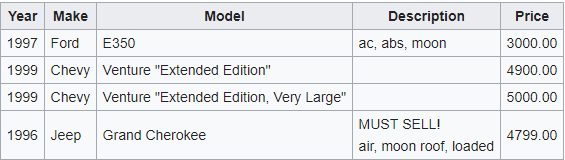
\includegraphics[width=0.6\textwidth]{figures/1174083_bakti/contohCSV1.png}}
		\caption{Contoh file}
		\label{Contoh CSV}
		\centerline{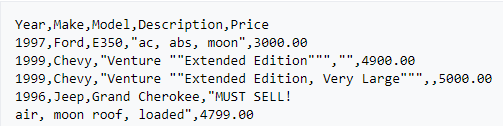
\includegraphics[width=0.6\textwidth]{figures/1174083_bakti/contohCSV2.png}}
		\caption{Contoh CSV}
		\label{Contoh CSV2}
	\end{figure}
\item Aplikasi-aplikasi apa saja yang bisa menciptakan file csv
	\begin{enumerate}
	\item Program Spreadsheet
			Seperti Microsoft Excel, Kspread, Staroffice Calc, OpenOffice Calc, Abacus, Gnumeric, WingZ, XESS.			
	\item Texteditor
			Seperti Notepad, Notepad++, Sublime, NetBeans, Adobe Dreamweaver, Visual Studio Code, dll 
	\end{enumerate}
	
\item Jelaskan bagaimana cara menulis dan membaca file csv di excel atau spreadsheet\\
\verb|		|Sesuai namanya, data atau nilai yang terdapat pada file CSV satu dengan yang lain dipisahkan dengan karakter koma (,). Jika berganti baris, maka itu dianggap record baru. Tentu saja ada kondisi tertentu yang harus dipenuhi agar file Excel bisa disimpan dalam format CSV. Setidaknya ada tiga kondisi utama yang harus dipenuhi, yaitu:
	\begin{itemize}
	\item Data yang diolah di Excel hanya berupa teks atau angka.
	\item Tidak mengandung VBA{Visual Basic for Application}.
	\item Hanya terdiri dari satu sheet.
	\end{itemize}
\paragraph{}Langkah untuk menyimpan file ke dalam format CSV cukup mudah, yaitu dengan memilih File $>$ Save As (Excel 2003 atau sebelumnya) atau dengan mengklik Microsoft Office Button $>$ Save As pada Excel 2007. Setelah itu pada kotak dialog yang muncul, pilihlah format CSV (Comma delimited) (*.csv) melalui drop-down Save as type.
\item Jelaskan sejarah library csv\\
\verb|		|CSV digunakan pada tahun 1983. untuk komputer Osborne Executive, yang membundel spreadsheet SuperCalc, mendokumentasikan konvensi kutipan CSV yang memungkinkan string mengandung koma yang disematkan, tetapi manual tersebut tidak menentukan konvensi untuk menanamkan tanda kutip dalam string yang dikutip. Daftar nilai yang dipisahkan dengan koma lebih mudah untuk diketik daripada data yang selaras dengan kolom tetap, dan cenderung menghasilkan hasil yang salah jika suatu nilai dieksekusi satu kolom dari lokasi yang dituju.
	
\item Jelaskan sejarah library pandas\\
\verb|		|Pengembangnya ialah Wes McKinney, mulai mengerjakan pandas pada 2008 ketika di AQR Capital Management karena kebutuhan akan alat kinerja tinggi yang fleksibel untuk melakukan analisis kuantitatif pada data keuangan. Sebelum meninggalkan AQR, dia bisa meyakinkan manajemen untuk mengizinkannya membuka sumber perpustakaan. Pegawai AQR lainnya, Chang She, bergabung dengan proyek ini pada 2012 sebagai kontributor utama kedua ke perpustakaan. Pada 2015, pandas menandatangani sebagai proyek NumFOCUS yang disponsori secara fiskal, sebuah badan amal nirlaba 501(c)(3) di Amerika Serikat.
	
\item Jelaskan fungsi-fungsi yang terdapat di library csv\\
\begin{itemize}
\item csv.reader\\
	\verb|		|Berfungsi untuk membaca dan mengembalikan data kedalam variable dari file csv.	Fungsi 	reader dirancang untuk mengambil data pada setiap baris didalam file dan membuat daftar semua 	kolom. Kemudian, tinggal dipilih kolom mana yang diinginkan untuk data variabel.
\lstinputlisting[firstline=12, lastline=24]{src/1174083/1174083_csv.py}

\item csv.writer\\
	\verb|		|Berfungsi untuk menuliskan data dari variable kedalam file csv. Fungsi writer akan membuat objek yang cocok untuk menulis. Untuk mengulang data yang ada di atas baris, gunakan fungsi writerow.
\lstinputlisting[firstline=39, lastline=45]{src/1174083/1174083_csv.py}
	
\item csv.register\textunderscore dialect untuk Mendaftarkan dialect pada csv
\item csv.unregister\textunderscore dialect untuk Menghapus dialect yang diasosiasi dengan nama dari registry dialect
\item csv.list\textunderscore dialects untuk Mengembalikan dialect yang diasosiasi dengan nama
\item csv.field\textunderscore size\textunderscore limit Mengembalikan ukuran field maksimum yang diizinkan oleh parser.
\item csv.DictReader\\
	\verb|		|Berfungsi untuk membaca dan mengembalikan data kedalam variable dictionary dari file csv.
\lstinputlisting[firstline=26, lastline=37]{src/1174083/1174083_csv.py}
\end{itemize}

\item Jelaskan fungsi-fungsi yang terdapat di library pandas\\
\begin{itemize}
	\item pandas.read\textunderscore csv\\
\verb|		|Berfungsi untuk membaca dan mengembalikan data kedalam format DataFrame dari file csv.
\lstinputlisting[firstline=47, lastline=50]{src/1174083/1174083_csv.py}
	\item to\textunderscore csv\\
\verb|		|Berfungsi untuk mengedit data didalam csv dan menulisnya kedalam file csv
\lstinputlisting[firstline=52, lastline=59]{src/1174083/1174083_csv.py}

\end{itemize}

\end{enumerate}

%%%%%%%%%%%%%%%%%%%%%%%%%%%%%%%%%%%%%%%%%%%%%%%%%%%%%%%%%%%%%%%%%%%%%%%%%%%%%%%%%%%%%%%%%%%%%%%%%%%%%%

\section{Ilham Muhammad Ariq D4TI2C 1174087}
\subsection{Pemahaman Teori}
\begin{enumerate}
    \item Apa itu fungsi file csv, jelaskan sejarah dan contoh
	
	\begin{itemize}
	\item Sejarah dan Fungsi
	\end{itemize}
	\par Comma Separated Values (CSV) adalah format data yang memberi tanggal lebih awal pada komputer pribadi lebih dari satu dekade: kompiler IBM Fortran (level H extended) di bawah OS / 360 mendukungnya pada tahun 1972. Input / output daftar-diarahkan ("bentuk bebas") didefinisikan dalam FORTRAN 77, disetujui pada tahun 1978. Input yang diarahkan daftar menggunakan koma atau spasi untuk pembatas, sehingga string karakter yang tidak dikutip tidak dapat mengandung koma atau spasi.
	
	\par Daftar nilai yang dipisahkan dengan koma lebih mudah untuk diketik (misalnya ke dalam kartu berlubang) daripada data yang selaras dengan kolom tetap, dan cenderung menghasilkan hasil yang salah jika suatu nilai ditinju satu kolom dari lokasi yang dituju.
	
	\par File CSV digunakan untuk pertukaran informasi basis data antara mesin dari dua arsitektur yang berbeda. Karakter teks-polos dari file CSV sebagian besar menghindari ketidakcocokan seperti urutan byte dan ukuran kata. File-file ini sebagian besar dapat dibaca oleh manusia, sehingga lebih mudah untuk mengatasinya tanpa adanya dokumentasi atau komunikasi yang sempurna.
	
	\par Inisiatif standardisasi utama - mentransformasikan "definisi fuzzy de facto" menjadi definisi yang lebih tepat dan de jure - adalah pada tahun 2005, dengan RFC4180, mendefinisikan CSV sebagai Tipe Konten MIME. Kemudian, pada 2013, beberapa kekurangan RFC4180 ditangani oleh rekomendasi W3C. 
	
	\par Pada 2014 IETF menerbitkan RFC7111 yang menjelaskan aplikasi fragmen URI pada dokumen CSV. RFC7111 menentukan bagaimana rentang baris, kolom, dan sel dapat dipilih dari dokumen CSV menggunakan indeks posisi.

	\par Pada 2015 W3C, dalam upaya untuk meningkatkan CSV dengan semantik formal, mempublikasikan draft rekomendasi pertama untuk standar metadata CSV, yang dimulai sebagai rekomendasi pada bulan Desember tahun yang sama. 
		      
    \item Aplikasi-aplikasi apa saja yang bisa menciptakan file csv?
   	beberapa aplikasi yang dapat menciptakan file dengan format csv antara lain 
   	\begin{itemize}
   	\item Microsoft Office  
   	\item Notepad 
   	\item UltraEdit
   	\item MySql
   	\item Oracle  			
   	\item OpenOffice
   	\item Spyder, dll
   	\end{itemize}
   
	\item Jelaskan bagaimana cara menulis dan membaca file csv di excel atau spreadsheet
		\begin{enumerate}
		\item Cara menulis	 
        \begin{itemize}
        \item Buat dokumen baru di Excel.
        \item Tambahkan judul kolom untuk setiap potongan informasi yang ingin dicatat (misalnya nama depan, nama belakang, alamat email, nomor telepon, dan ulang tahun), lalu ketikkan informasi dalam kolom yang sesuai.
        \item Setelah selesai, Pilih File lalu Simpan Sebagai.
        \item Gunakan kotak menurun untuk memilih CSV (Berbatas koma) (.csv), beri nama pada file, lalu pilih Simpan.
   	    \end{itemize}
        \item Cara membaca
        \begin{itemize}
        \item Buka MS Excel Anda.
        \item Klik Data lalu Get External Data lalu From Text.
        \item Akan muncul Text Import Wizard, arahkan pada file csv yang ingin anda buka lalu Open.
        \item Setelah File terbuka, akan muncul Text Import Wizard Step 1 lalu Pilih Delimited, Kemudian Next (Di sini, bisa juga menentukan baris awal yang akan di import), Step 2 lalu Centang pada Tab dan Comma (Atau sesuai pengaturan File Anda) lalu Next, Step 3 lalu Atur Format data pada tiap kolom yang tampil dan klik Finish.
        \item File anda sudah tertata rapi dan dapat di baca dengan mudah melalui MS Excel 2007
    \end{itemize}	
	\end{enumerate}
	
	\item Jelaskan sejarah library csv
	
	CSV muncul untuk memudahkan data science dan analis karena dinilai terdapat banyak kemudahan yang didapat. CSV dapat dimaksimalkan jika dipaduka dengan python karena python adalah bahasa pemrograman yang support ke banyak library termasuk csv. Maka karena itulah perpaduan python dan csv seringkali digunakan oleh perusahaan-perushaan besar dalam mengolah datanya.
	
	\item Jelaskan sejarah library pandas

	Pandas merupakan toolkit yang powerfull sebagai alat analisis data dan struktur untuk bahasa pemrograman Python. Dengan menggunakan pandas kita dapat mengolah data dengan mudah, salah satu fiturnya adalah Dataframe. Dengan adanya fitur dataframe kita dapat membaca sebuah file dan menjadikannya tabble, kita juga dapat mengolah suatu data dengan menggunakan operasi seperti join, distinct, group by, agregasi, dan teknik lainnya yang terdapat pada SQL. Banyak format file yang dapat dibaca menggunakan Pandas, seperti file .txt, .csv, .tsv dan lainnya. Agar lebih jelas mari kita mencobanya secara langsung.
	
	\item Jelaskan fungsi-fungsi yang terdapat di library csv
	ada 2 fungsi pada csv :
	\begin{enumerate}
	\item Fungsi membaca library csv
		
	\lstinputlisting[firstline=8, lastline=20]{src/1174087/1174087_csv.py}
		
	\item Fungsi menulis library csv
		
	\lstinputlisting[firstline=8, lastline=14]{src/1174087/1174087_csv1.py}
	\end{enumerate}

	\item Jelaskan fungsi-fungsi yang terdapat di library pandas
			ada 2 fungsi pada pandas :
	\begin{enumerate}
	\item Fungsi membaca library pandas
		
	\lstinputlisting[firstline=8, lastline=10]{src/1174087/1174087_csv2.py}
		
	\item Fungsi menulis library pandas
		
	\lstinputlisting[firstline=8, lastline=13]{src/1174087/1174087_csv3.py}
	\end{enumerate}
		
\end{enumerate}   

%%%%%%%%%%%%%%%%%%%%%%%%%%%%%%%%%%%%%%%%%%%%%%%%%%%%%%%%%%%%%%%%%%%%%%%%%%%%%%%%%%%%%%%%%%%%%%%%%%%%%%%%%%%%%%%%%


\section{Muhammad Abdul Gani Wijaya}
\subsection{Teori CSV}
\begin{enumerate}
\item Apa fungsi file csv? Jelaskan sejarah dan contoh !\\
Jawaban :

\begin{itemize}
\item Fungsi File CSV
\end{itemize}

Comma Separated Value atau CSV adalah format data yang memudahkan penggunanya melakukan penginputan data ke database secara sederhana. CSV bisa digunakan dalam standar file ASCII, di mana setiap record dipisahkan dengan tanda koma atau titik koma.

\begin{itemize}
\item Sejarah CSV
\end{itemize}

Dari rilis pertama, Excel menggunakan format file biner yang disebut Binary Interchange File Format (BIFF) sebagai format file utamanya. Ini berubah ketika Microsoft merilis Office System 2007 yang memperkenalkan Office Open XML sebagai format file utamanya. Office Open XML adalah file kontainer berbasis XML yang mirip dengan XML Spreadsheets (XMLSS), yang diperkenalkan di Excel 2002. File versi XML tidak bisa menyimpan makro VBA.

Meskipun mendukung format XML baru, Excel 2007 masih mendukung format lama yang masih berbasis BIFF tradisional. Selain itu Microsoft Excel juga mendukung format Comma Separated Values (CSV), DBase File (DBF), SYMbolic LinK (SYLK), Format Interchange Data (DIF) dan banyak format lainnya, termasuk format lembar kerja 1-2 Lotus - 3 (WKS, WK1, WK2, dll.) Dan Quattro Pro.


\begin{itemize}
\item Contoh File CSV
\begin{verbatim}
Nama,Umur, Alamat
Muhammad Abdul Gani Wijaya, 19 Tahun, Jl. Isekai
\end{verbatim}
\end{itemize}


\item Aplikasi apa aja yang dapat membuat file csv\\
Jawaban :

\begin{itemize}
\item Microsoft Excel
\item Google Spreadsheet
\item Notepad ++
\item Text Editor lainnya
\end{itemize}

\item  Bagaimana ara menulis dan membaca file csv di excel atau spreadsheet\\
Jawaban :

\begin{itemize}
\item Cara Menulis file csv
\end{itemize}
Berikut adalah kode untuk menulis file CSV dengan menggunakan built-in module csv yang dimiliki Python

\begin{verbatim}
import csv

siswa = [
    ('Shinmei', 'A', 95),
    ('Da Lopez', 'B', 90),
    ('Nurhadi', 'A', 80),
    ('Captain Marvel', 'B', 90),
    ('Thanos', 'C', 70)
]

# tentukan lokasi file, nama file, dan inisialisasi csv
f = open('siswa.csv', 'w')
w = csv.writer(f)
w.writerow(('Nama','Kelas','Nilai'))

# menulis file csv
for s in siswa:
    w.writerow(s)

# menutup file csv
f.close()
\end{verbatim}


\item Sejarah library csv\\
Jawaban :\\
 library pandas dibuat agar bahasa pemograman python bisa bersaing R dan matlab, yang digunakan untuk mengolah banyak data , keperluan big data, data mining data science dan sebagainya.

\item Sejarah library pandas\\
Jawaban :\\
Library csv dibuat untuk permudah mengolah data. Dan mempermudah untuk melakukan export dan import file csv itu sendiri


\item Jelaskan  fungsi-fungsi yang terdapat di library csv\\
Jawaban :\\
Terdapat 2 fungsi dari library csv, yaitu :

\begin{itemize}
\item Cara membaca file
\end{itemize}
import csv

tentukan lokasi file, nama file, dan inisialisasi csv
f = open('siswa.csv', 'r')
reader = csv.reader(f)

membaca baris per baris
for row in reader:
    print row

menutup file csv
f.close()

\begin{itemize}
\item Cara menulis file
\end{itemize}
Nama,Kelas,Nilai
arslan,A,90
bayu,B,85
niko,A,80
abdul,B,90
dahlan,C,70

\item Jelaskan  fungsi-fungsi yang terdapat di library pandas\\
Jawaban :\\
Library pandas penulisannya lebih sederhana dan terlihat lebih rapih dari pada library csv.


\end{enumerate}


%%%%%%%%%%%%%%%%%%%%%%%%%%%%%%%%%%%%%%%%%%%%%%%%%%%%%%%%%%%%%%%%%%%%%%%%%%%%%%%%%%%%%%%%%%%%

\section{Muhammad Reza Syachrani / 1174084}
\subsection{Pemahaman Teori}
\begin{enumerate}
    \item CSV adalah Comma Separated Values suatu format data dalam basis data di mana setiap record dipisahkan dengan tanda koma (,) atau titik koma (;). Selain sederhana, format ini dapat dibuka dengan berbagai text-editor seperti Notepad, Wordpad, bahkan MS Excel.
    \par File CSV (Nilai Berbatas Koma) adalah tipe file khusus yang dapat Anda buat atau edit di Excel. File CSV menyimpan informasi yang dipisahkan oleh koma, bukan menyimpan informasi dalam kolom. Saat teks dan angka disimpan dalam file CSV, mudah untuk memindahkannya dari satu program ke program lain. Misalnya, Anda dapat mengekspor kontak dari Google ke dalam file CSV, kemudian mengimpornya ke Outlook.
    \item Aplikasi-aplikasi yang bisa menciptakan file CSV antara lain adalah notepad++, visual studio code, atom, sublime, excell, google spreadshare, dan LibreOfficecalc.
    \item Cara menulis file csv di excel atau spreadsheet
    \begin{enumerate}
        \item Buat dokumen baru di Excel.
        \item Tambahkan judul kolom untuk setiap potongan informasi yang ingin dicatat (misalnya nama depan, nama belakang, alamat email, nomor telepon, dan ulang tahun), lalu ketikkan informasi dalam kolom yang sesuai.
        \item Setelah selesai, Pilih File > Simpan Sebagai.
        \item Gunakan kotak menurun untuk memilih CSV (Berbatas koma) (*.csv), beri nama pada file, lalu pilih Simpan
    \end{enumerate}
    \par Sedangkan cara membaca file csv di excel atau spreadsheet
    \begin{enumerate}
        \item klik data - get external data - form text
        \item Text Import Wizard, arahkan pada file csv lalu Open
        \item Setelah File terbuka, akan muncul Text Import Wizard.
        \item Pilih Delimited, Kemudian Next (Di sini, bisa juga menentukan baris awal yang akan di import)
        \item Centrang pada Tab dan Comma (Atau sesuai pengaturan File Anda) lalu Next.
        \item Atur Format data pada tiap kolom yang tampil dan klik Finish
    \end{enumerate}
    \item Sejarah Library CSV  dibuat untuk mepermudah mengolah data dan mempermudah untuk melakukan export dan import file CSV.
    \item Sejarah library pandas dibuat untuk bahasa pemograman python agar bisa bersaing dengan  R dan matlab, yang digunakan untuk mengolah banyak data , keperluan big data, data mining, dan data science.
    \item fungsi-fungsi yang terdapat di library CSV
    \begin{itemize}
        \item Reading CSV
        \par csv.reader digunakan untuk Membaca dari file CSV dilakukan menggunakan objek pembaca. File CSV dibuka sebagai file teks dengan fungsi open () built-in Python, yang mengembalikan objek file.
        \item Writing CSV
        \par csv.writer digunakan untuk dapat menulis ke file CSV.
    \end{itemize}
    \item fungsi-fungsi yang terdapat di library pandas
    \begin{itemize}
        \item Reading CSV
        \par pandas.read\_csv digunakan untuk membuka, menganalisis, dan membaca file CSV yang disediakan, dan menyimpan data dalam DataFrame.
        \item Writing CSV
        \par  Menulis DataFrame ke file CSV semudah membaca. contoh membuat variabel df yang menggunakan pandas.read\_csv setelah itu menambahkan fungsi to\_csv () pada varibel df untuk memberikan nama file.
    \end{itemize}
    
\end{enumerate}

%%%%%%%%%%%%%%%%%%%%%%%%%%%%%%%%%%%%%%%%%%%%%%%%%%%%%%%%%%%%%%%%%%%%%%%%%%%%%%
\section{Advent Nopele Olansi Damiahan Sihite || 1174089}
\subsection{Teori}
\begin{enumerate}

\item Apa itu fungsi file csv, jelaskan sejarah dan contoh\\
Jawaban :

\begin{itemize}
\item Fungsi File CSV
\end{itemize}

Comma Separated Value atau CSV adalah format data yang memudahkan penggunanya melakukan penginputan data ke database secara sederhana. CSV bisa digunakan dalam standar file ASCII, di mana setiap record dipisahkan dengan tanda koma atau titik koma.


\begin{itemize}
\item Contoh file csv
\begin{verbatim}
Nama,Umur, Alamat
Advent Nopele Olansi Damiahan Sihite, 19 Tahun, Jl. sarimanah
\end{verbatim}
\end{itemize}

\item Aplikasi yang dapat membuat file csv\\
Jawaban :

\begin{itemize}
\item Microsoft Excel
\item Google Spreadsheet
\item Notepad ++
\item Text Editor lainnya
\end{itemize}

\item  Cara menulis dan membaca file csv di excel atau spreadsheet\\
Jawaban :

\begin{itemize}
\item Cara Menulis file csv
\end{itemize}
Berikut adalah kode untuk menulis file CSV dengan menggunakan built-in module csv yang dimiliki Python

\begin{verbatim}
import csv

siswa = [
    ('arslan', 'A', 90),
    ('bayu', 'B', 85),
    ('niko', 'A', 80),
    ('abdul', 'B', 90),
    ('dahlan', 'C', 70)
]

# tentukan lokasi file, nama file, dan inisialisasi csv
f = open('siswa.csv', 'w')
w = csv.writer(f)
w.writerow(('Nama','Kelas','Nilai'))

# menulis file csv
for s in siswa:
    w.writerow(s)

# menutup file csv
f.close()
\end{verbatim}

\begin{itemize}
\item Cara membaca file csv
\end{itemize}

Berikut adalah contoh kode untuk membaca file CSV 

\begin{verbatim}
import csv

# tentukan lokasi file, nama file, dan inisialisasi csv
f = open('siswa.csv', 'r')
reader = csv.reader(f)

# membaca baris per baris
for row in reader:
    print row

# menutup file csv
f.close()
\end{verbatim}

\item Sejarah library pandas\\
Jawaban :\\
library csv dibuat untuk bahasa pemograman python agar bisa bersaing dengan  R dan matlab, yang digunakan untuk mengolah banyak data , keperluan big data, data mining, dan data science.

\item Sejarah library csv\\
Jawaban :\\
library pandas dibuat untuk mepermudah mengolah data dan mempermudah untuk melakukan export dan import file CSV.

\item Jelaskan  fungsi-fungsi yang terdapat di library csv\\
Jawaban :\\
Terdapat 2 fungsi dari library csv, yaitu :

\begin{itemize}
\item Cara membaca file
\end{itemize}

\begin{itemize}
\item Cara menulis file
\end{itemize}
Di Python, hasil pembacaan setiap baris pada file CSV akan dikonversi menjadi list Python.

\item Jelaskan  fungsi-fungsi yang terdapat di library pandas\\
Jawaban :\\
library pandas penulisannya lebih sederhana dan terlihat lebih rapih dari pada library csv.

\end{enumerate}
%%%%%%%%%%%%%%%%%%%%%%%%%%%%%%%%%%%%%%%%%%%%%%%%%%%%%%%%%%%%%%%%%%%%%%%

\bibliographystyle{IEEEtran} 
%\def\bibfont{\normalsize}
\bibliography{references}


%%%%%%%%%%%%%%%
%%  The default LaTeX Index
%%  Don't need to add any commands before \begin{document}
\printindex

%%%% Making an index
%% 
%% 1. Make index entries, don't leave any spaces so that they
%% will be sorted correctly.
%% 
%% \index{term}
%% \index{term!subterm}
%% \index{term!subterm!subsubterm}
%% 
%% 2. Run LaTeX several times to produce <filename>.idx
%% 
%% 3. On command line, type  makeindx <filename> which
%% will produce <filename>.ind 
%% 
%% 4. Type \printindex to make the index appear in your book.
%% 
%% 5. If you would like to edit <filename>.ind 
%% you may do so. See docs.pdf for more information.
%% 
%%%%%%%%%%%%%%%%%%%%%%%%%%%%%%

%%%%%%%%%%%%%% Making Multiple Indices %%%%%%%%%%%%%%%%
%% 1. 
%% \usepackage{multind}
%% \makeindex{book}
%% \makeindex{authors}
%% \begin{document}
%% 
%% 2.
%% % add index terms to your book, ie,
%% \index{book}{A term to go to the topic index}
%% \index{authors}{Put this author in the author index}
%% 
%% \index{book}{Cows}
%% \index{book}{Cows!Jersey}
%% \index{book}{Cows!Jersey!Brown}
%% 
%% \index{author}{Douglas Adams}
%% \index{author}{Boethius}
%% \index{author}{Mark Twain}
%% 
%% 3. On command line type 
%% makeindex topic 
%% makeindex authors
%% 
%% 4.
%% this is a Wiley command to make the indices print:
%% \multiprintindex{book}{Topic index}
%% \multiprintindex{authors}{Author index}

\end{document}

